\documentclass[12pt,a4paper]{report}
\usepackage[utf8]{inputenc}
\usepackage[french]{babel}
\usepackage[T1]{fontenc}
\usepackage{graphicx}
\usepackage{hyperref}
\usepackage{geometry}
\geometry{margin=2.5cm}

\setcounter{secnumdepth}{3}
\setcounter{tocdepth}{3}
\usepackage{float}
\usepackage{listings}
\usepackage{xcolor}
\usepackage{tabularx}
\lstset{
    basicstyle=\ttfamily\small,
    breaklines=true,
    frame=single,
    columns=fullflexible,
    keepspaces=true
}


\usepackage{booktabs}
\usepackage{array}

\usepackage{enumitem}
\usepackage[most]{tcolorbox}
\usepackage{tikz}
\usetikzlibrary{arrows.meta,positioning,shapes.geometric,fit,calc}

\begin{document}
\begin{titlepage}
\centering

{\Large RÉPUBLIQUE ALGÉRIENNE DÉMOCRATIQUE ET POPULAIRE}\\[0.5cm]
{\large MINISTÈRE DE LA DÉFENSE NATIONALE}\\[0.3cm]
{\large ÉCOLE MILITAIRE POLYTECHNIQUE}\\[2cm]

\begin{figure}[h!]
\centering

\begin{minipage}{0.45\textwidth}
    \centering
    
\includegraphics[width=\linewidth]{./images/unita.png}
\end{minipage}
\hfill
\begin{minipage}{0.45\textwidth}
    \centering
    
\includegraphics[width=\linewidth]{./images/ecrmt.png}
\end{minipage}

\end{figure}

\vspace{1cm}

{\Huge \textbf{Rapport de stage}\par}

\vspace{0.8cm}

{\Large
Conception et développement d’une application web de gestion et de suivi du courrier\par
}

\vspace{1.5cm}

\begin{flushleft}
\textbf{Réalisé par :}\\[0.2cm]
EOC. Ait Ikhlef Lyes\\
EOC. HADDAD Nour-El-Islem \\[1cm]

\textbf{Encadré par :}\\[0.2cm]
Cdt. Boutemjet Yacine \\
\end{flushleft}

\vfill

{\large Année Universitaire 2025--2026\par}

\end{titlepage}
\tableofcontents
uhjuhu
\newpage
\listoffigures
\newpage
\chapter*{Remerciements}
\addcontentsline{toc}{chapter}{Remerciements}

Nous tenons tout d’abord à remercier Allah le tout-puissant et miséricordieux, qui nous a donné la force, la patience, la volonté et le courage pour la réussite dans nos études. En second lieu, nous tenons à témoigner nos vifs remerciements à nos encadreurs Commandant «Boutemjet Yacine» et Mme «Menacer Meriem»  pour leur précieux conseils et leur aide durant toute la période du travail, et tous les officiers du laboratoire central de recherche et développement
pour leurs conseils judicieux, leur aide et leur disponibilité. Nos vifs remerciements vont également aux membres du jury pour l’intérêt qu’ils ont porté à notre travail en acceptant de l’examiner et de l’enrichir par leurs propositions. Enfin, nous tenons également à remercier toutes les personnes qui ont participé de près ou de loin à la réalisation de ce travail.

%==================== TABLE ====================




% ================= INTRODUCTION =================

\include{presentaion_unite}
\chapter{Etude de l'existant et proposition de solution}

\section*{Introduction}

Ce chapitre présente d'abord le problème rencontré dans la gestion du courrier administratif. Il décrit ensuite le système existant basé sur Redmine, ses apports et ses limites. Enfin, il propose une solution web dédiée, mieux adaptée au suivi, à la validation, à la transmission et à l'archivage des courriers.
\section{Problématique}
\label{sec:problematique}

La gestion du courrier paraît, au premier abord, comme une tâche assez simple : recevoir un document, l’enregistrer, le transmettre à la personne concernée, puis le classer. Pourtant, dans une organisation où plusieurs services interviennent, les choses deviennent rapidement moins évidentes. Un même courrier peut passer par plusieurs responsables, attendre une validation, être renvoyé vers un autre service ou rester bloqué faute de suivi clair.

Avec l’augmentation des échanges numériques, le problème devient encore plus visible. Les courriers, les pièces jointes et les réponses s’accumulent dans plusieurs espaces. Certains documents sont conservés dans les boîtes de réception, d’autres dans des dossiers partagés, parfois même sur les postes des utilisateurs. À ce moment-là, retrouver un courrier précis ou connaître son état réel demande souvent du temps.

Un autre problème se pose au niveau du suivi. Lorsqu’un courrier doit être validé ou traité par plusieurs personnes, il n’est pas toujours facile de savoir qui l’a consulté, qui doit répondre, ou à quelle étape il se trouve. Cette situation peut provoquer des retards, des oublis ou même une perte d’information, surtout lorsque les méthodes de classement changent d’un utilisateur à un autre.

La confidentialité des documents représente aussi un point sensible. Les courriers administratifs peuvent contenir des informations importantes ou personnelles. S’ils sont mal transmis, mal classés ou accessibles à des personnes non concernées, cela peut créer des risques pour l’organisation.

Ces difficultés montrent que la gestion du courrier ne peut pas se limiter à un simple échange de messages ou à un stockage de fichiers. Elle demande un système plus organisé, capable de suivre les documents depuis leur création jusqu’à leur archivage, tout en respectant les rôles des utilisateurs et les étapes de validation.

\section{Étude du système de gestion de courrier actuel}
\label{sec:etude_existant}

Le système existant est basé sur Redmine, installé à l’aide de la stack Bitnami. Bitnami facilite l’installation de Redmine en regroupant les éléments nécessaires à son fonctionnement dans un seul environnement \cite{bitnami_redmine}. Redmine est une application web de gestion de projet écrite avec Ruby on Rails. Il propose notamment le suivi des demandes, les rôles, les workflows, les documents, les fichiers, le wiki et les notifications par email \cite{redmine_overview}.

Dans le système actuel, le courrier est traité avec la logique de Redmine. Ce fonctionnement peut aider pour suivre une demande ou une tâche, mais il reste moins adapté à un courrier administratif. Un courrier ne passe pas seulement d’un état à un autre : il peut être reçu, enregistré, transmis, validé, retourné, répondu puis archivé. Redmine permet bien de gérer des statuts et des transitions dans ses workflows \cite{redmine_workflow}, mais cette logique reste orientée vers le suivi d’\textit{issues} plutôt que vers le cycle complet d’un document administratif.

\begin{figure}[ht]
  \centering
  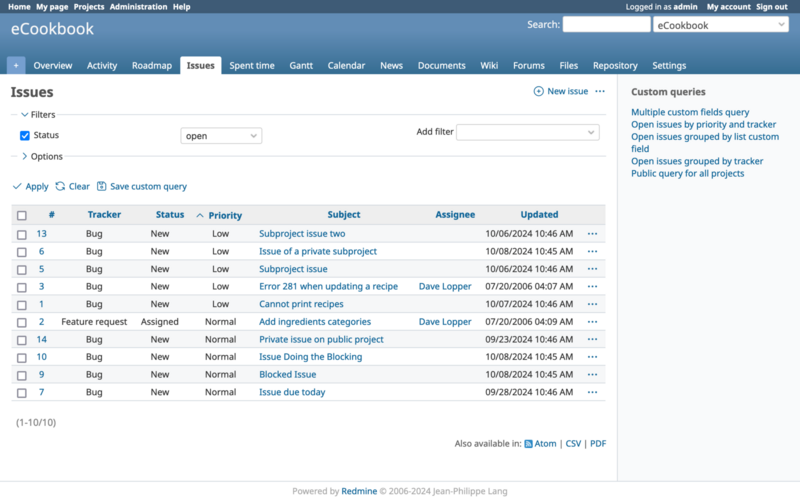
\includegraphics[width=0.9\textwidth]{images/redmin/redmine_interface.png}
  \caption{Interface du système actuel basé sur Redmine \cite{redmineup_themes_2025}.}
  \label{fig:redmine_ui}
\end{figure}

Redmine possède aussi une API REST qui donne accès à certaines ressources et permet des opérations de base comme la création, la modification ou la suppression. Cette API supporte les formats XML et JSON \cite{redmine_rest_api}. Malgré cela, le besoin de notre projet dépasse la simple gestion d’une demande. Il faut suivre le parcours du courrier, gérer les validations, faciliter la recherche, notifier les utilisateurs concernés et garder une trace claire des actions.
\begin{figure}[t]
  \centering
  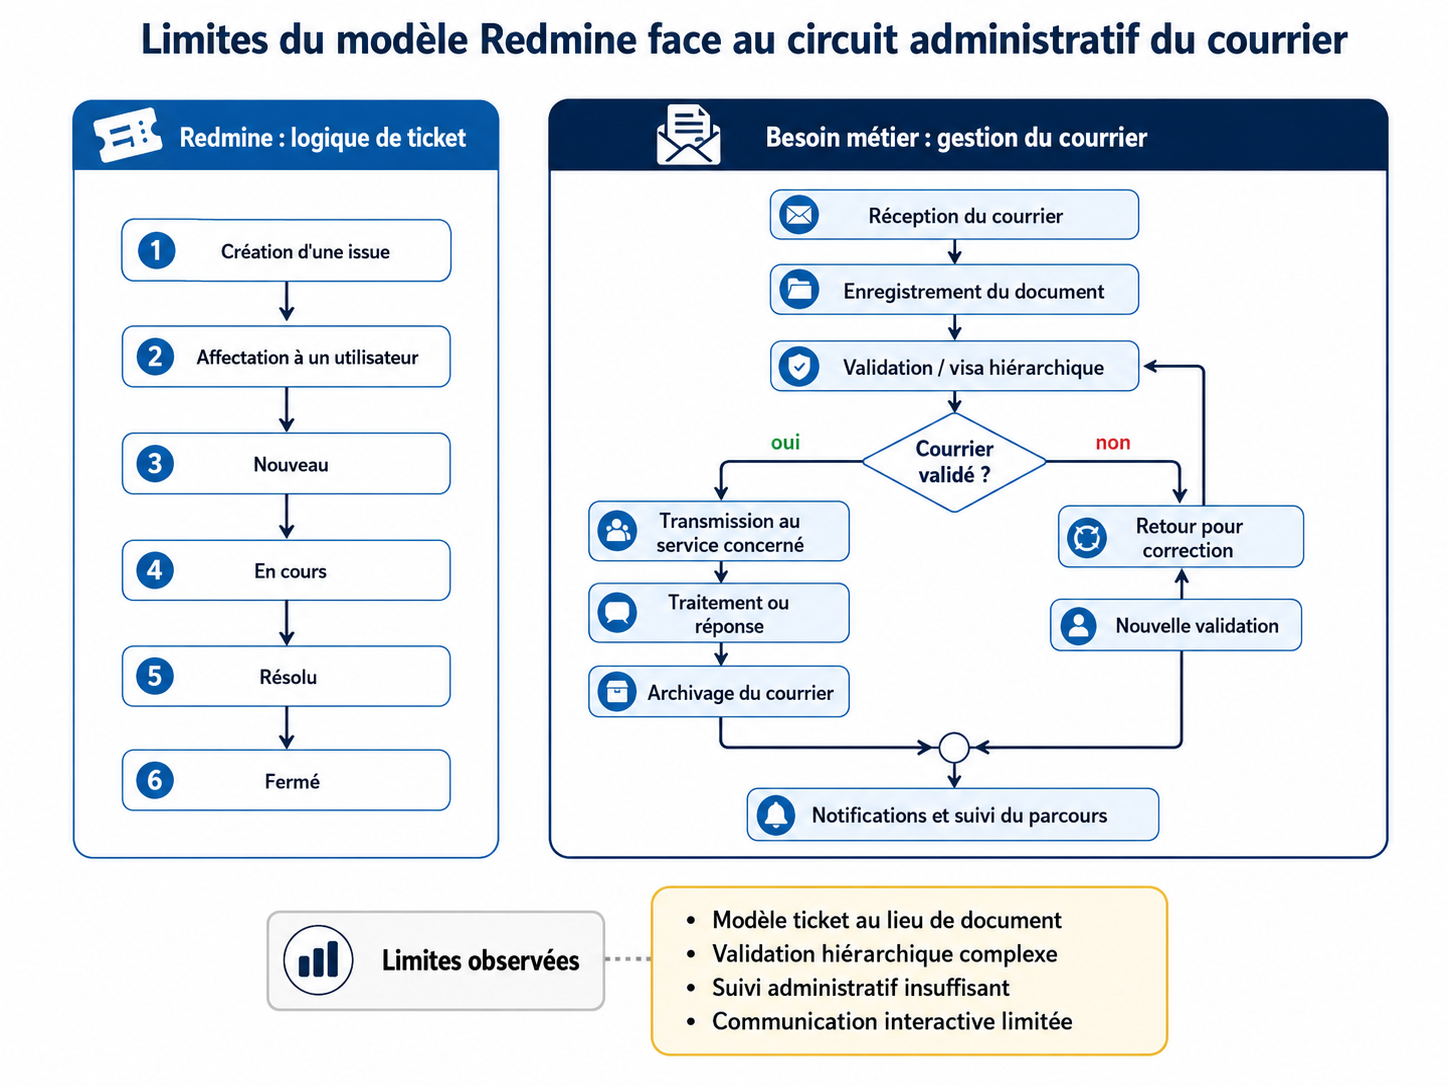
\includegraphics[width=0.95\textwidth]{images/redmin/limites_redmine_courrier.png}
  \caption{Comparaison entre le modèle Redmine et le circuit de gestion du courrier voulus}
  \label{fig:limites_schema}
\end{figure}

Redmine reste donc utile pour la gestion de projet et le suivi des tâches, mais il ne répond pas entièrement aux besoins d’une gestion de courrier. Les limites les plus visibles concernent la logique documentaire, la validation hiérarchique, le suivi des transmissions et la communication en temps réel. Ces limites expliquent le choix de développer une application dédiée à la gestion du courrier.


\section{Proposition de solution}
\label{sec:proposition_solution}

Pour améliorer cette situation, nous proposons de développer une application web dédiée à la gestion du courrier. Cette solution vise à regrouper les courriers, les pièces jointes et les échanges dans un même espace, afin d’éviter la dispersion des informations entre plusieurs outils ou dossiers.

L’application permettra d’enregistrer les courriers entrants et sortants, de les transmettre aux services concernés et de suivre leur avancement. Chaque utilisateur accédera aux fonctions liées à son rôle, ce qui permettra de mieux organiser les responsabilités entre les agents, les secrétaires et les responsables.

Le système prendra aussi en charge les validations hiérarchiques. Ainsi, lorsqu’un courrier nécessite l’avis ou l’approbation d’un responsable, son parcours pourra être suivi plus clairement. Les utilisateurs concernés seront informés des actions à effectuer, ce qui réduira les risques d’oubli ou de retard.

La solution proposée intégrera également la gestion des pièces jointes, les notifications, l’archivage et l’historique des actions réalisées sur chaque courrier. De cette manière, il sera plus simple de savoir qui a traité un document, quand il a été transmis et dans quel état il se trouve.

Cette application devrait donc rendre la circulation du courrier plus claire, réduire les manipulations répétitives et faciliter la recherche des informations. Elle permettra aussi d’améliorer le suivi administratif des documents au sein de l’organisation.
\section*{Conclusion}

Cette étude montre que le système actuel facilite certains aspects du suivi, mais ne couvre pas entièrement les besoins liés au courrier administratif. La solution proposée permet de mieux organiser le traitement des documents, de clarifier les responsabilités et d'assurer un suivi plus fiable depuis la création du courrier jusqu'à son archivage.

\chapter{Généralités sur le courrier}
\label{chap:generalites_courrier}

\section{Introduction}
\label{sec:introduction_generalites_courrier}

Le courrier, qu’il soit traditionnel ou électronique, reste un moyen important pour échanger des informations entre les personnes, les entreprises et les administrations. Avec l’évolution des technologies numériques, le courrier électronique a pris une place très large dans les échanges quotidiens. Il permet d’envoyer rapidement des messages, des documents et des informations sans avoir besoin d’un support papier. Malgré cette facilité, son utilisation demande une bonne organisation, car les messages reçus et envoyés peuvent vite devenir nombreux et difficiles à gérer. C’est pour cette raison que la gestion du courrier électronique est devenue nécessaire pour assurer un meilleur suivi, une bonne conservation et une communication plus claire.

\begin{figure}[H]
    \centering
    % Image à chercher : évolution du courrier papier vers le courrier électronique
    % Exemple : lettre papier, ordinateur, symbole e-mail, Internet
    %\includegraphics[width=0.75\textwidth]{images/evolution_courrier.png}
    \caption{Évolution du courrier traditionnel vers le courrier électronique}
    \label{fig:evolution_courrier}
\end{figure}

\section{Définition du courrier}
\label{sec:definition_courrier}

Le courrier électronique, appelé aussi \textit{courriel}, est un moyen de communication numérique qui permet d’échanger des informations à travers un système de messagerie. Il peut être utilisé entre particuliers, dans les entreprises ou dans les administrations. Il sert à transmettre un message, mais aussi des fichiers joints, comme des documents, des images ou des formulaires \cite{bissonnette2012}.

D’un point de vue organisationnel, un courriel ne se limite pas seulement au texte envoyé. Il comprend aussi les pièces jointes et les métadonnées, comme l’expéditeur, le destinataire, l’objet, la date et l’heure d’envoi \cite{piaf}. Ces éléments sont importants, car ils permettent de mieux comprendre le contexte du message et de le conserver correctement.



\section{Défis de la gestion du courrier}
\label{sec:defis_gestion_courrier}

Dans une entreprise, la gestion des courriels n’est pas toujours simple. Avec le grand nombre de messages envoyés chaque jour, il devient parfois difficile de retrouver rapidement une information ou de bien organiser les échanges. Certains utilisateurs gardent tous leurs courriels sans les classer, ce qui surcharge les boîtes de messagerie et complique le travail au fil du temps \cite{piafgestion}.

Des problèmes de confidentialité peuvent aussi apparaître. Un message électronique peut être transféré ou copié en quelques secondes, parfois à des personnes qui ne sont pas directement concernées. Il arrive également que des documents importants soient supprimés par erreur, alors que d’autres restent stockés inutilement pendant plusieurs années \cite{piafgestion}.

Les difficultés ne concernent pas uniquement l’organisation des messages. Les outils de messagerie utilisés dans la plupart des organisations ne sont pas conçus spécialement pour l’archivage des documents. Selon Natalie Bissonnette, certains formats de sauvegarde comme HTML ou PST ne garantissent pas toujours une bonne conservation des informations liées au courriel, notamment les métadonnées \cite{bissonnette2012}. Pour cette raison, plusieurs organismes préfèrent utiliser le format PDF/A afin de conserver les courriels dans de meilleures conditions \cite{bissonnette2012}.

La manière de gérer les courriels change aussi d’une personne à une autre. Certains utilisateurs classent correctement leurs messages, alors que d’autres utilisent simplement leur boîte de réception pour conserver tous leurs documents. Cette différence dans les pratiques peut provoquer des pertes d’informations et rendre le repérage des fichiers plus compliqué \cite{piafgestion}.

\begin{figure}[H]
    \centering
    % Image à chercher : boîte mail surchargée ou gestion difficile des courriels
    % Contenu souhaité : plusieurs e-mails, notifications, surcharge, dossiers non classés
    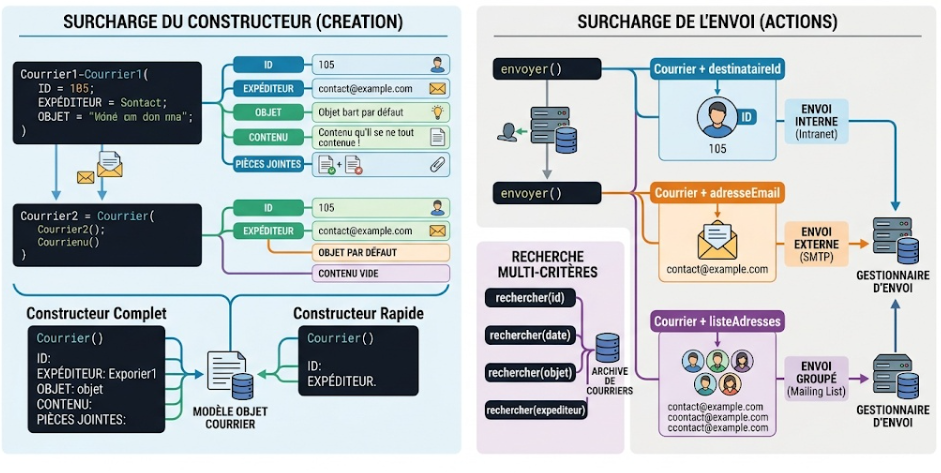
\includegraphics[width=0.75\textwidth]{images/courrier/deff.png}
    \caption{Exemple de surcharge dans la gestion des courriels}
    \label{fig:defis_gestion_courrier}
\end{figure}

\section{Importance du courrier électronique}
\label{sec:importance_courrier}

Le courrier électronique occupe une place importante dans le fonctionnement des entreprises et des administrations. Il permet d’échanger rapidement des informations, d’envoyer des documents et de garder une trace écrite des communications. Grâce à cette rapidité, plusieurs tâches peuvent être réalisées sans déplacement ni attente prolongée \cite{bissonnette2012}.

Dans le cadre professionnel, le courriel sert souvent à transmettre des décisions, des demandes, des contrats ou encore des informations liées au suivi des activités. Certains messages peuvent même avoir une valeur juridique ou administrative lorsqu’ils prouvent qu’une action a été effectuée ou qu’une décision a été prise \cite{bissonnette2012}. Pour cette raison, les organisations doivent accorder une attention particulière à leur conservation et à leur classement.

Le courrier électronique facilite aussi le travail collaboratif. Plusieurs personnes peuvent recevoir le même message, partager des fichiers ou suivre l’évolution d’un projet en temps réel. Selon Techno-Science, ce moyen de communication est apprécié pour sa rapidité, son faible coût et la possibilité d’envoyer différents types de documents numériques \cite{technoscience}.

Cependant, l’importance du courriel ne se limite pas seulement à la communication. Il joue également un rôle dans la mémoire de l’organisation. Certains échanges permettent de retracer des décisions, de comprendre le contexte d’un projet ou de conserver des informations utiles sur une longue période \cite{bissonnette2012}. C’est pour cette raison que plusieurs organismes mettent en place des politiques de gestion et d’archivage des courriels afin d’éviter les pertes d’informations et d’assurer une meilleure organisation documentaire.

\begin{figure}[H]
    \centering
    % Image à chercher : communication professionnelle par e-mail
    % Contenu souhaité : employés, ordinateur, échange de documents,
    % collaboration, messagerie professionnelle
    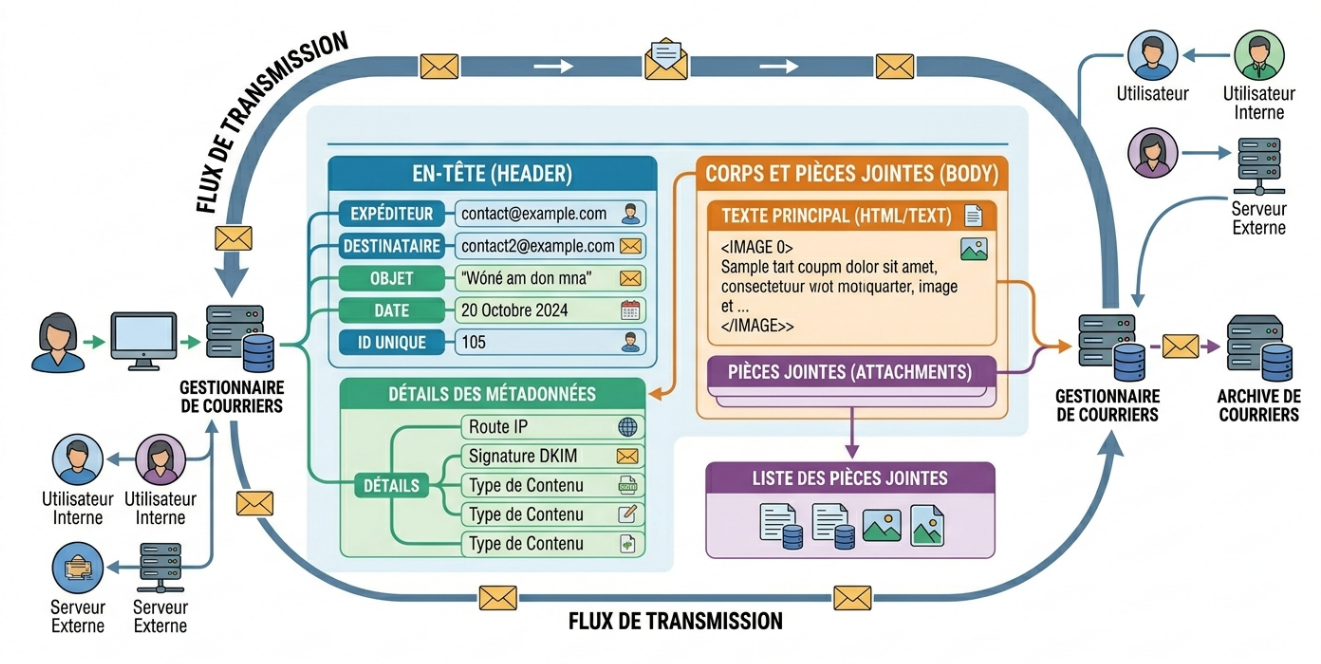
\includegraphics[width=0.75\textwidth]{images/courrier/image.png}
    \caption{Le courrier électronique dans la communication professionnelle}
    \label{fig:importance_courriel}
\end{figure}


\section{Conclusion}
\label{sec:conclusion_generalites_courrier}

Dans ce chapitre, nous avons présenté les notions générales liées au courrier électronique ainsi que son rôle dans les échanges professionnels et administratifs. Le courriel facilite la communication et le partage rapide des informations, ce qui explique son utilisation dans presque toutes les organisations.

Nous avons aussi vu que la gestion des courriels ne se limite pas seulement à l’envoi et à la réception des messages. Elle concerne également le classement, la conservation et la sécurité des informations échangées. Plusieurs difficultés peuvent apparaître, surtout lorsque les messages sont nombreux ou mal organisés.

Enfin, les applications de gestion de courrier permettent d’améliorer le suivi des échanges et de réduire les risques de perte d’informations. Le chapitre suivant sera consacré à l’étude et à la conception de notre application de gestion de courrier électronique.

\label{chap:generalitecourrier}

\chapter{Généralités UML et Conception du système}
\label{chap:conception}

\section{Le langage UML}
\label{sec:langage_uml}

\subsection{Définition}
\label{subsec:definition_uml}

UML, ou \textit{Unified Modeling Language}, se définit comme un langage de modélisation graphique et textuel destiné à comprendre et décrire des besoins, spécifier, concevoir des solutions et communiquer des points de vue. Il ne s’agit pas d’une simple notation graphique, car les concepts transmis par un diagramme ont une sémantique précise et sont porteurs de sens au même titre que les mots d’un langage.

UML permet de visualiser, spécifier, construire et documenter les éléments d’un système logiciel \cite{omg_uml_spec}. Il est aussi utilisé pour modéliser la structure, le comportement et l’architecture des applications, ainsi que les processus métier et les structures de données \cite{omg_uml}. Dans notre projet, UML est utilisé pour exprimer les besoins et décrire la conception de notre application de gestion de courrier.

\subsection{Caractéristiques d’UML}
\label{subsec:caracteristiques_uml}

Dans le cadre de la modélisation d’une application informatique, UML possède plusieurs caractéristiques importantes.

Tout d’abord, UML n’est pas une méthode ou un processus. Il ne définit pas l’enchaînement complet des activités de développement, mais il fournit un langage permettant de représenter les différents aspects d’un système. Le choix de la démarche reste donc indépendant du langage UML.

Ensuite, UML est un langage semi-formel. Il repose sur des concepts de modélisation ayant une signification précise. Cela permet de réduire les ambiguïtés et de faciliter la compréhension entre les membres d’une équipe de projet.

UML possède aussi une représentation graphique standardisée. Cette notation commune permet aux analystes, développeurs et autres intervenants de lire les mêmes diagrammes avec une compréhension proche.

Enfin, UML offre plusieurs vues complémentaires d’un système. Chaque diagramme présente une partie différente : les besoins, les acteurs, les échanges, les classes, les états ou encore l’architecture technique. Cette séparation aide à mieux maîtriser la complexité d’un système.

\subsection{Les points forts et faibles d’UML}
\label{subsec:points_forts_faibles_uml}

\subsubsection{Les points forts d’UML}
\label{subsubsec:points_forts_uml}

UML est un langage formel et normalisé. Il permet de gagner en précision, d’encourager l’utilisation d’outils de modélisation et de garder une documentation claire du système. Son caractère visuel facilite aussi la communication entre les différents acteurs du projet.

UML est également un bon support de communication. Il cadre l’analyse et facilite la compréhension de représentations parfois abstraites. Grâce à ses différents diagrammes, il devient plus simple d’expliquer le fonctionnement général d’une application avant de passer au développement.

Par rapport à Merise, UML est plus adapté à la conception orientée objet. Il permet de représenter à la fois les données, les traitements, les interactions et le comportement du système. Merise reste utile pour les systèmes fortement centrés sur les données, mais UML est souvent plus souple pour les applications web modernes, où les objets métier, les interfaces et les échanges évoluent ensemble.

\subsubsection{Les points faibles d’UML}
\label{subsubsec:points_faibles_uml}

La mise en pratique d’UML demande un apprentissage. Il faut comprendre le rôle de chaque diagramme et savoir lequel utiliser selon le besoin. Si tous les diagrammes sont utilisés sans nécessité, la conception peut devenir lourde.

UML ne remplace pas non plus une méthode de gestion de projet. Il permet de modéliser le système, mais il ne dit pas exactement comment organiser toutes les étapes du développement. Il doit donc être utilisé avec une démarche claire, en choisissant seulement les diagrammes utiles pour le projet.

\section{Conception du système}
\label{sec:conception_systeme}

Dans cette section, nous présentons les différents diagrammes réalisés pour la conception de notre application.

\subsection{Étude préliminaire}
\label{subsec:etude_preliminaire}

Avant de présenter les différents diagrammes de conception, nous réalisons une étude préliminaire afin d’identifier les acteurs qui interagissent avec le système ainsi que les principales fonctionnalités offertes par l’application.

\subsubsection{Identification des acteurs}
\label{subsubsec:identification_acteurs}

Les principaux acteurs du système sont :

\begin{itemize}
    \item \textbf{Agent} : consulte les courriers qui lui sont destinés et répond aux courriers nécessitant une réponse.
    \item \textbf{Secrétaire} : consulte, répond et transmet les courriers liés à son organe.
    \item \textbf{Secrétaire générale} : crée et suit les courriers reçus au niveau de l’établissement.
    \item \textbf{Chef d’organe} : valide, transmet et suit les courriers de son organe.
    \item \textbf{Chef général} : supervise le traitement global des courriers et valide les courriers au niveau de l’établissement.
    \item \textbf{Administrateur} : gère les utilisateurs, le référentiel et la configuration du système.
\end{itemize}

\subsubsection{Identification des fonctionnalités}
\label{subsubsec:identification_fonctionnalites}

Les principales fonctionnalités du système sont :

\begin{itemize}
    \item l’authentification des utilisateurs ;
    \item la gestion des utilisateurs ;
    \item la création des courriers ;
    \item la consultation des courriers ;
    \item la transmission des courriers ;
    \item la validation des courriers ;
    \item la réponse aux courriers ;
    \item la recherche des courriers ;
    \item l’archivage des courriers ;
    \item l’administration du référentiel et de la configuration.
\end{itemize}
\subsection{Diagramme de classes}
\label{subsec:diagramme_classes}

\begin{figure}[h]
    \centering
    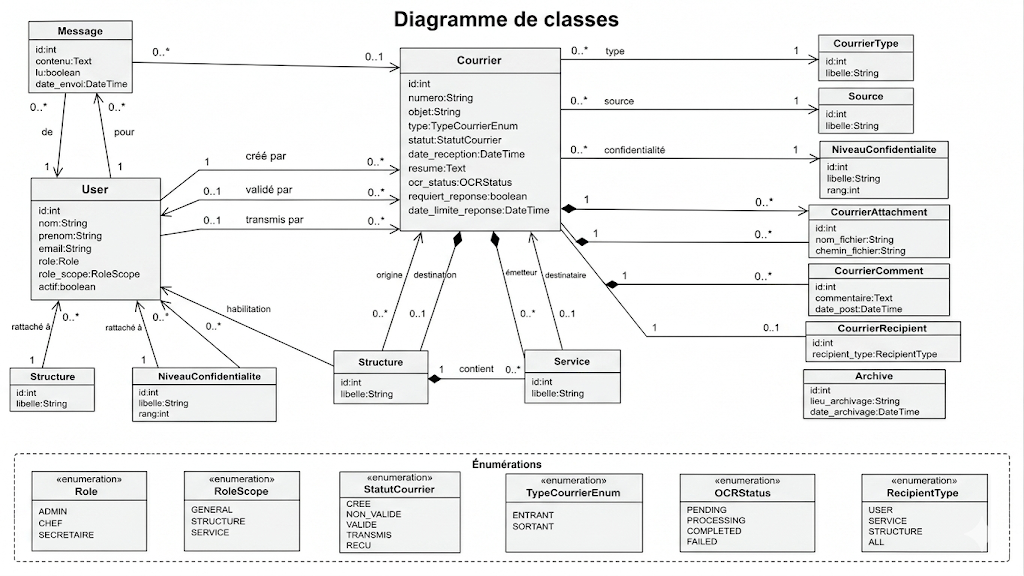
\includegraphics[width=\textwidth,height=0.85\textheight,keepaspectratio]{diagrams/classD/classD.png}
    \caption{Diagramme de classes de l’application}
    \label{fig:diagramme_classes}
\end{figure}

\subsection{Diagrammes de cas d’utilisation}
\label{subsec:diagrammes_cas_utilisation}

\subsubsection{Diagramme de cas d’utilisation global}
\label{subsubsec:cas_utilisation_global}

\begin{figure}[H]
    \centering
    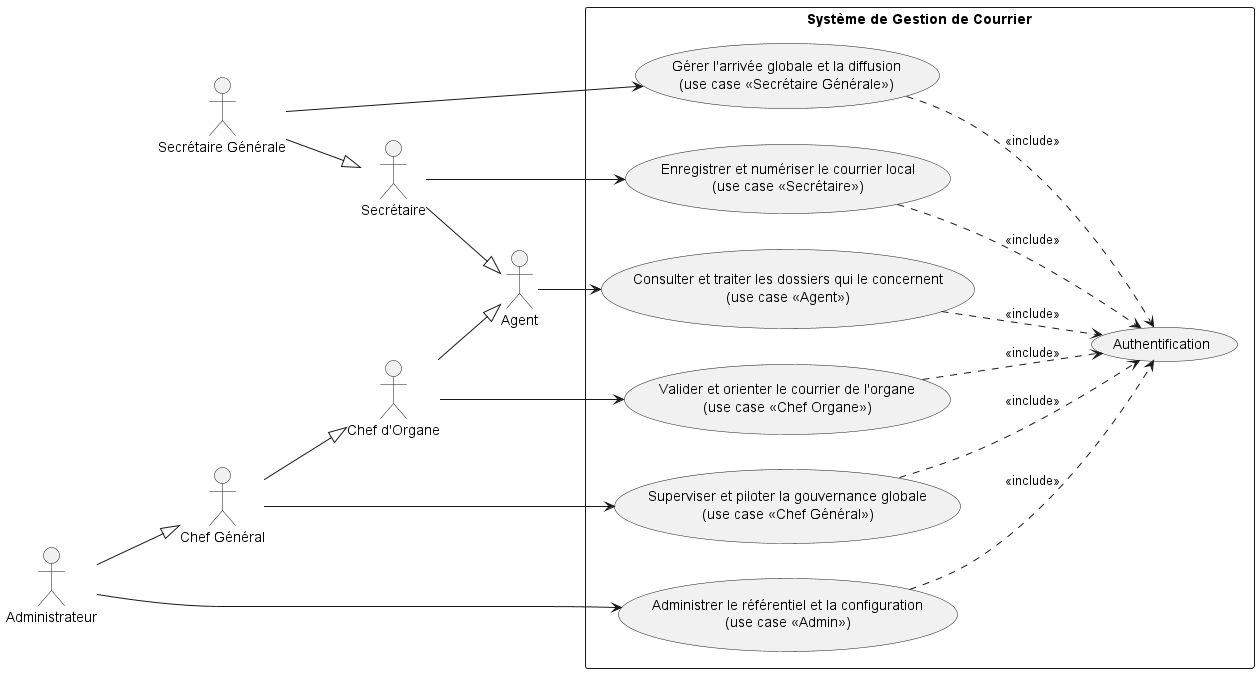
\includegraphics[width=14cm]{out/diagrams/usecases/puml/usecase_global/usecase_global.png}
    \caption{Diagramme de cas d’utilisation global}
    \label{fig:cas_utilisation_global}
\end{figure}

\subsubsection{Diagramme de cas d’utilisation de l’administrateur}
\label{subsubsec:cas_utilisation_admin}

\begin{figure}[H]
    \centering
    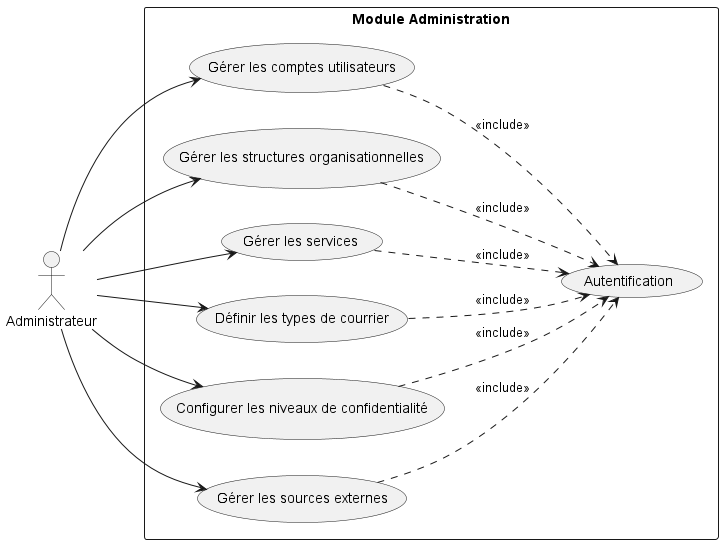
\includegraphics[width=14cm]{out/diagrams/usecases/puml/usecase_admin/usecase_admin.png}
    \caption{Diagramme de cas d’utilisation de l’administrateur}
    \label{fig:cas_utilisation_admin}
\end{figure}

\subsubsection{Diagramme de cas d’utilisation du chef général}
\label{subsubsec:cas_utilisation_chef_general}

\begin{figure}[H]
    \centering
    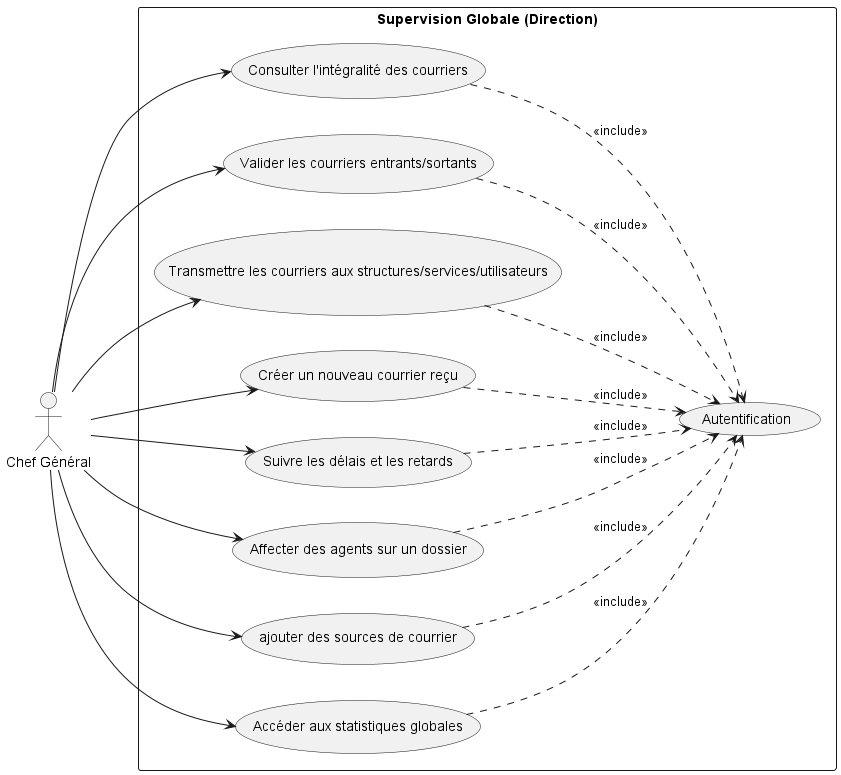
\includegraphics[width=14cm]{out/diagrams/usecases/puml/usecase_chef_general/usecase_chef_general.png}
    \caption{Diagramme de cas d’utilisation du chef général}
    \label{fig:cas_utilisation_chef_general}
\end{figure}

\subsubsection{Diagramme de cas d’utilisation de la secrétaire générale}
\label{subsubsec:cas_utilisation_secretaire_generale}

\begin{figure}[H]
    \centering
    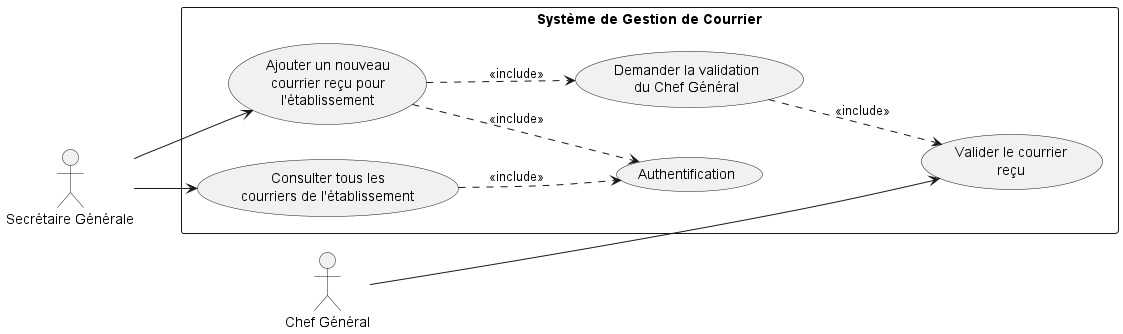
\includegraphics[width=14cm]{out/diagrams/usecases/puml/usecase_secretaire_general/usecase_secretaire_generale.png}
    \caption{Diagramme de cas d’utilisation de la secrétaire générale}
    \label{fig:cas_utilisation_secretaire_generale}
\end{figure}

\subsubsection{Diagramme de cas d’utilisation du chef d’organe}
\label{subsubsec:cas_utilisation_chef_organe}

\begin{figure}[H]
    \centering
    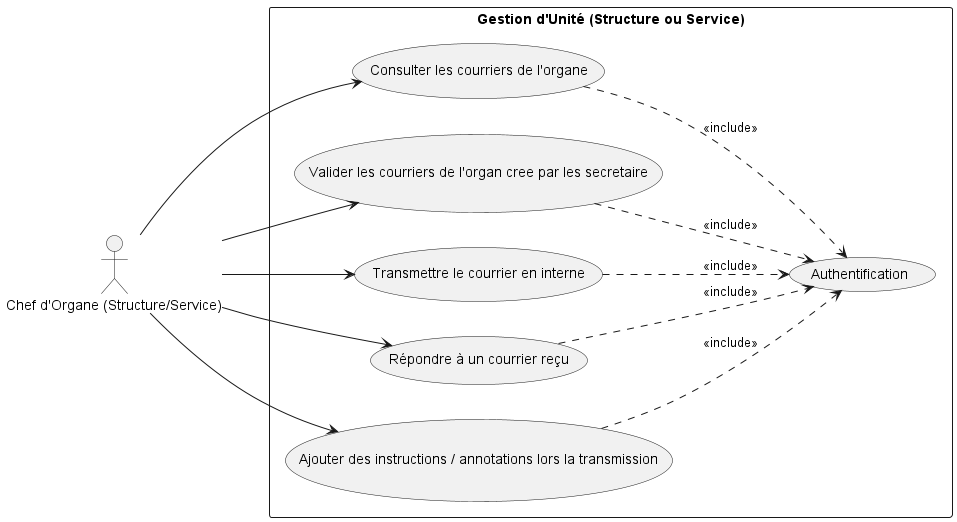
\includegraphics[width=14cm]{out/diagrams/usecases/puml/usecase_chef_organe/usecase_chef_organe.png}
    \caption{Diagramme de cas d’utilisation du chef d’organe}
    \label{fig:cas_utilisation_chef_organe}
\end{figure}
\subsubsection{Diagramme de cas d’utilisation de la secrétaire d’organe}
\label{subsubsec:cas_utilisation_secretaire_organe}

\begin{figure}[H]
    \centering
    
\includegraphics[width=14cm]{/mnt/c/Users/ENPEI/Desktop/courrier project/courier/out/diagrams/usecases/puml/usecase_secretaire/usecase_secretaire_organe.png}
    \caption{Diagramme de cas d’utilisation de la secrétaire d’organe}
    \label{fig:cas_utilisation_secretaire_organe}
\end{figure}
\subsubsection{Diagramme de cas d’utilisation de l’agent}
\label{subsubsec:cas_utilisation_agent}

\begin{figure}[H]
    \centering
    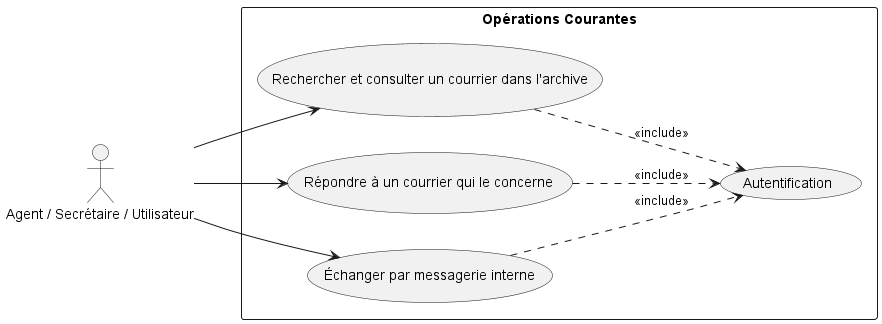
\includegraphics[width=14cm]{out/diagrams/usecases/puml/usecase_agent/usecase_agent.png}
    \caption{Diagramme de cas d’utilisation de l’agent}
    \label{fig:cas_utilisation_agent}
\end{figure}

\subsection{Diagrammes de séquence}
\label{subsec:diagrammes_sequence}

\subsubsection{Diagramme de séquence d’authentification}
\label{subsubsec:sequence_authentification}

\begin{figure}[H]
    \centering
    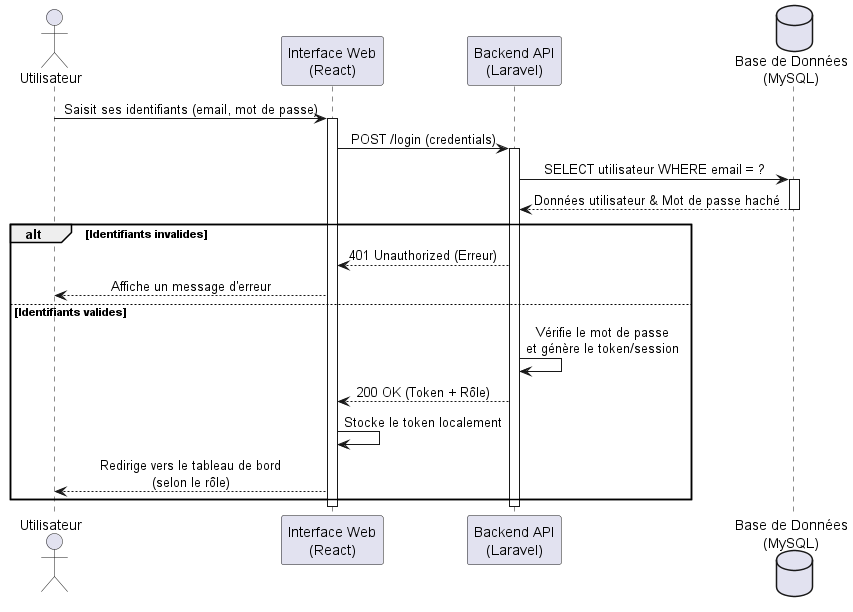
\includegraphics[width=14cm]{out/diagrams/seq_authentification/seq_authentification.png}
    \caption{Diagramme de séquence d’authentification}
    \label{fig:sequence_authentification}
\end{figure}

\subsubsection{Diagramme de séquence de création d’un courrier}
\label{subsubsec:sequence_creation_courrier}

\begin{figure}[H]
    \centering
    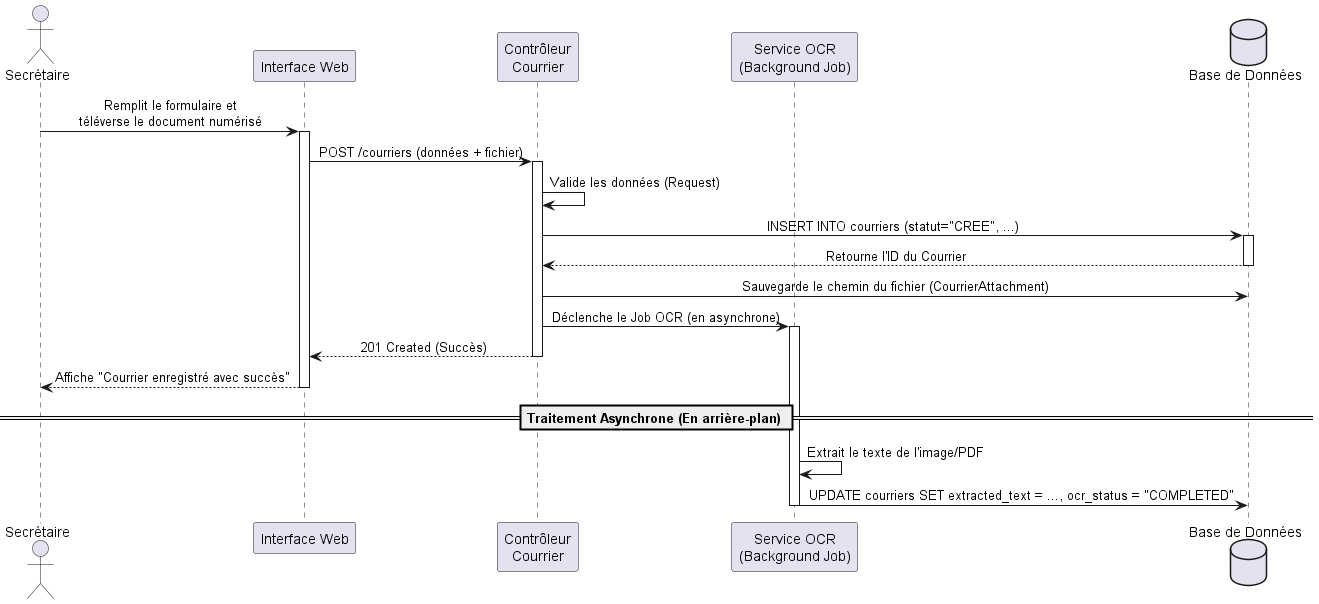
\includegraphics[width=14cm]{out/diagrams/seq_creation_courrier/seq_creation_courrier.png}
    \caption{Diagramme de séquence de création d’un courrier}
    \label{fig:sequence_creation_courrier}
\end{figure}

\subsubsection{Diagramme de séquence de transmission d’un courrier}
\label{subsubsec:sequence_transmission_courrier}

\begin{figure}[H]
    \centering
    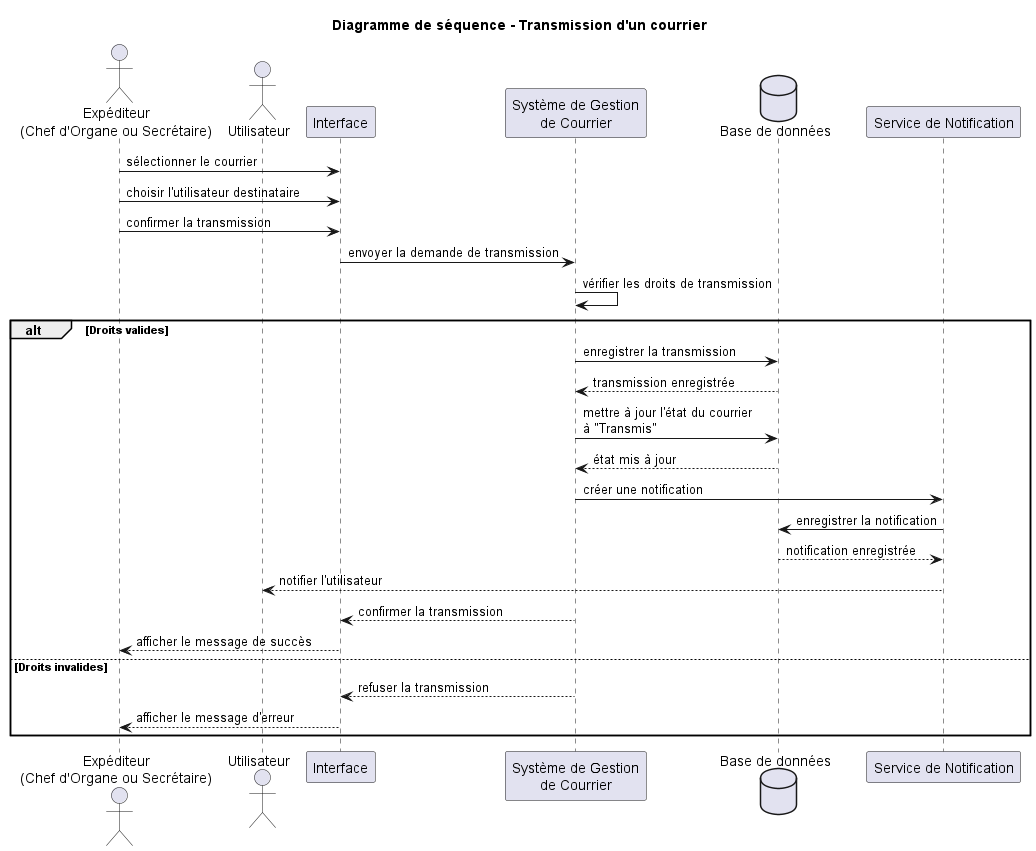
\includegraphics[width=14cm,height=0.5\textheight]{out/diagrams/seq_transmission_courrier/sequence_transmission_courrier.png}

    \caption{Diagramme de séquence de transmission d’un courrier}
    \label{fig:sequence_transmission_courrier}
\end{figure}

\subsubsection{Diagramme de séquence de réponse à un courrier}
\label{subsubsec:sequence_reponse_courrier}

\begin{figure}[H]
    \centering
    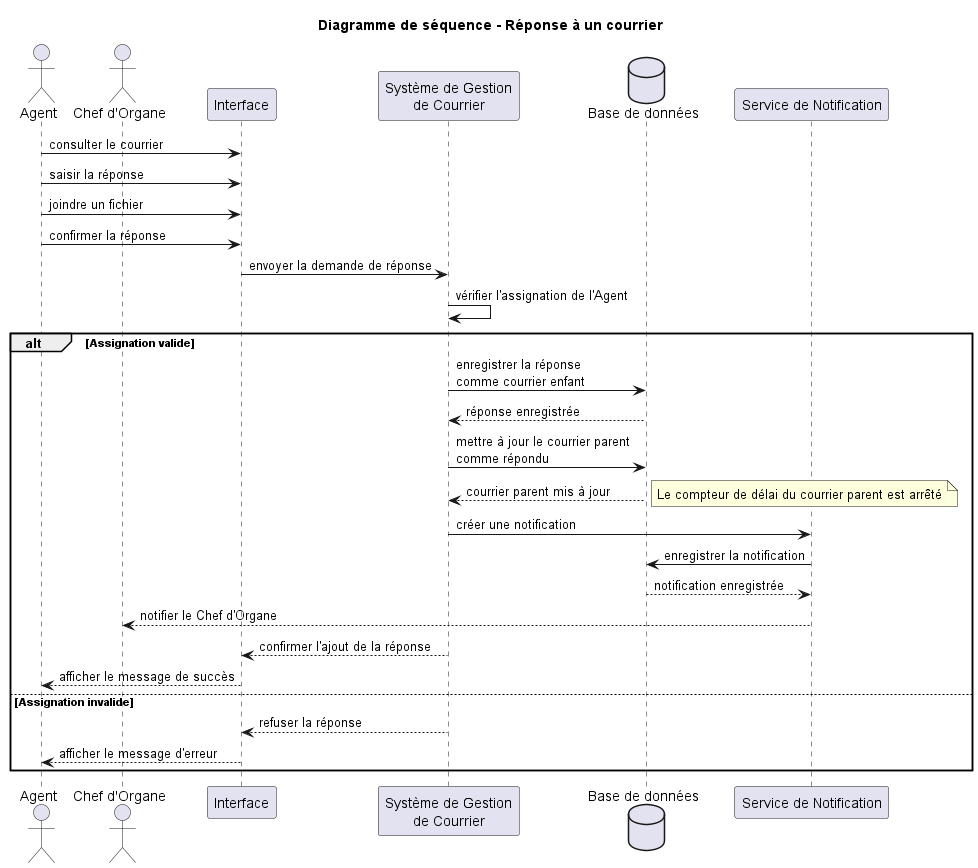
\includegraphics[width=14cm,height=0.3\textheight]{out/diagrams/seq_reponse_courrier/sequence_reponse_courrier.png}
    
    \caption{Diagramme de séquence de réponse à un courrier}
    \label{fig:sequence_reponse_courrier}
\end{figure}

\subsubsection{Diagramme de séquence d’archivage d’un courrier}
\label{subsubsec:sequence_archivage_courrier}

\begin{figure}[H]
    \centering
    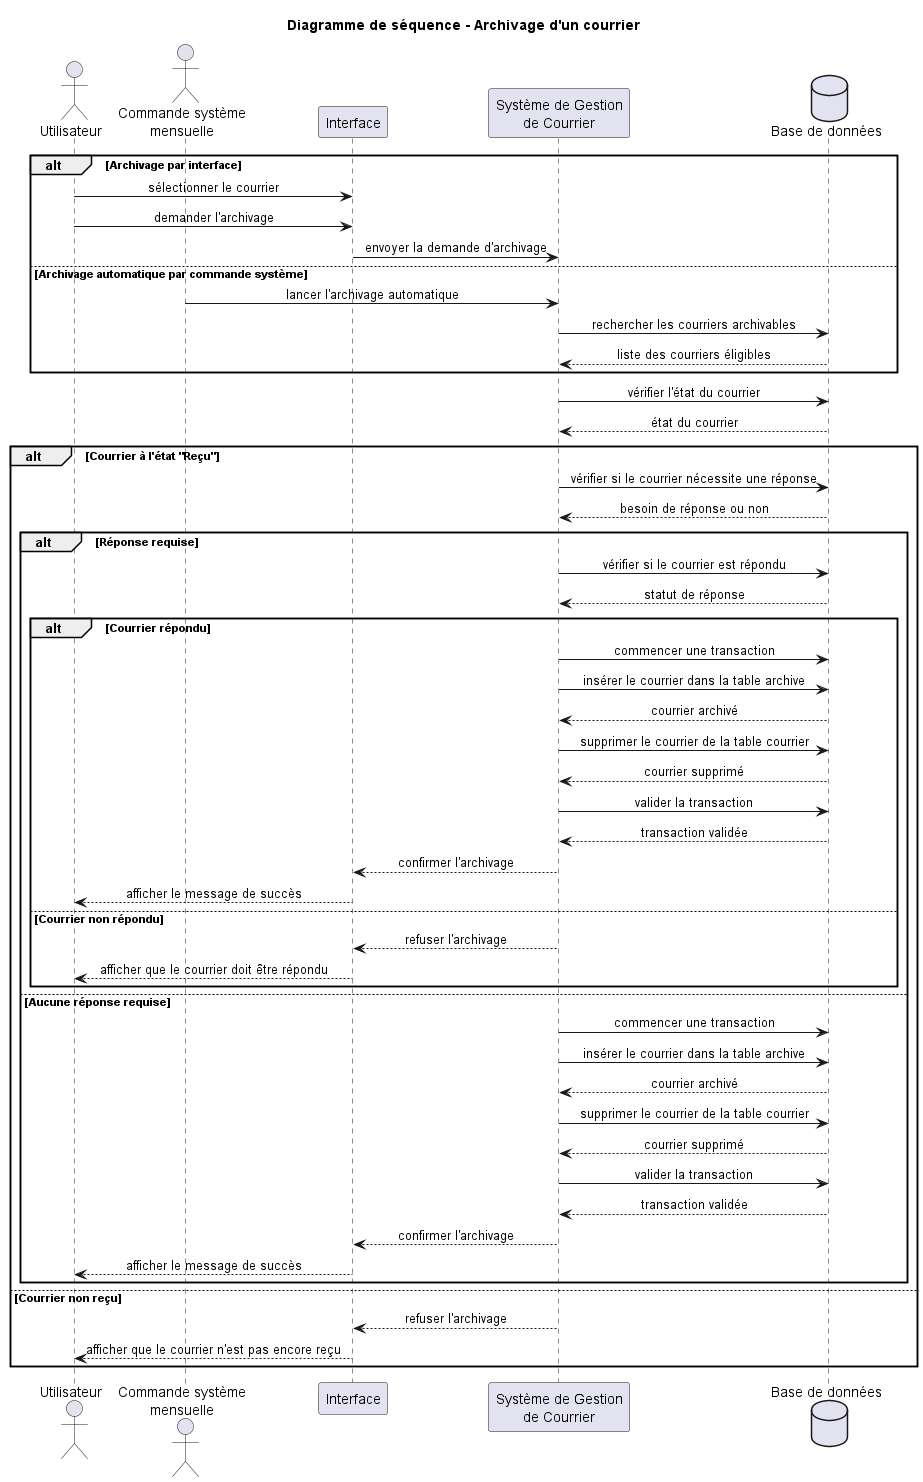
\includegraphics[width=0.90\textwidth,height=0.5\textheight]{out/diagrams/seq_archivage/sequence_archivage_courrier.png}
    \caption{Diagramme de séquence d’archivage d’un courrier}
    \label{fig:sequence_archivage_courrier}
\end{figure}

\subsubsection{Diagramme de séquence de recherche d’un courrier}
\label{subsubsec:sequence_recherche_courrier}

\begin{figure}[H]
    \centering
    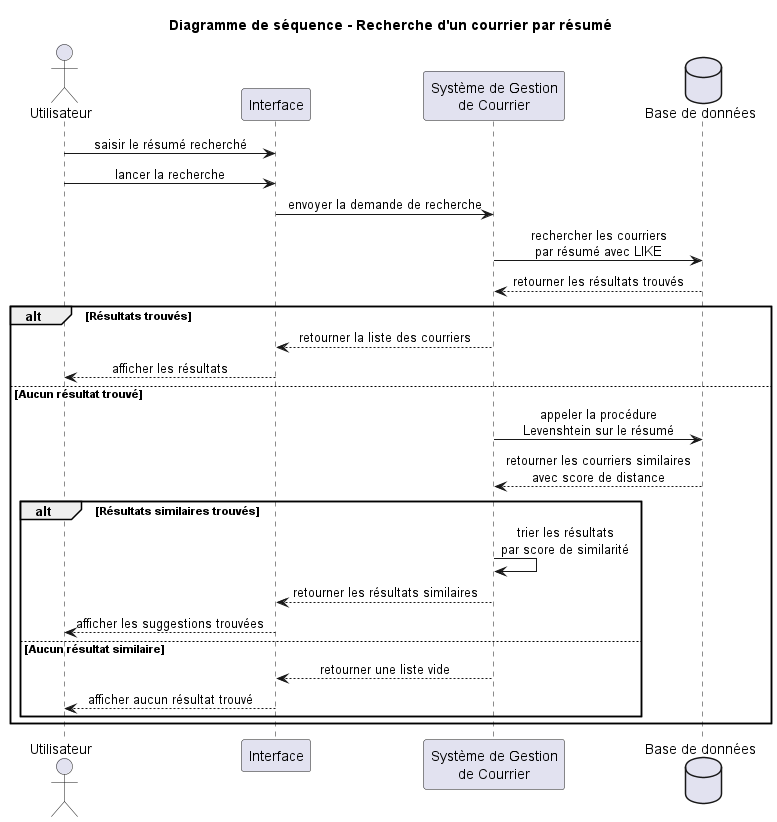
\includegraphics[width=0.90\textwidth,height=0.44\textheight]{out/diagrams/seq_recherche/sequence_recherche_courrier.png}
    \caption{Diagramme de séquence de recherche d’un courrier}
    \label{fig:sequence_recherche_courrier}
\end{figure}

\subsubsection{Diagramme de séquence de validation d’un courrier}
\label{subsubsec:sequence_validation_courrier}

\begin{figure}[H]
    \centering
    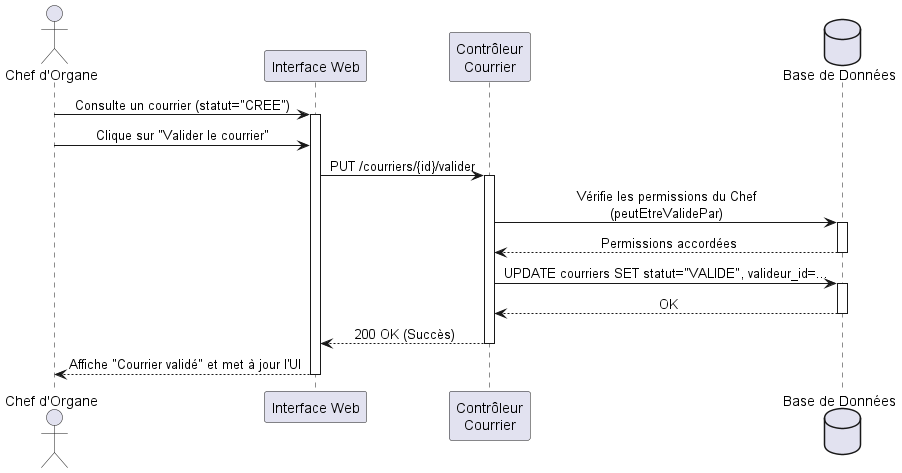
\includegraphics[width=14cm]{out/diagrams/seq_validation_courrier/seq_validation_courrier.png}
    \caption{Diagramme de séquence de validation d’un courrier}
    \label{fig:sequence_validation_courrier}
\end{figure}
\subsection{Diagramme d’états-transitions}
\label{subsec:diagramme_etats_transitions}

\begin{figure}[H]
    \centering
    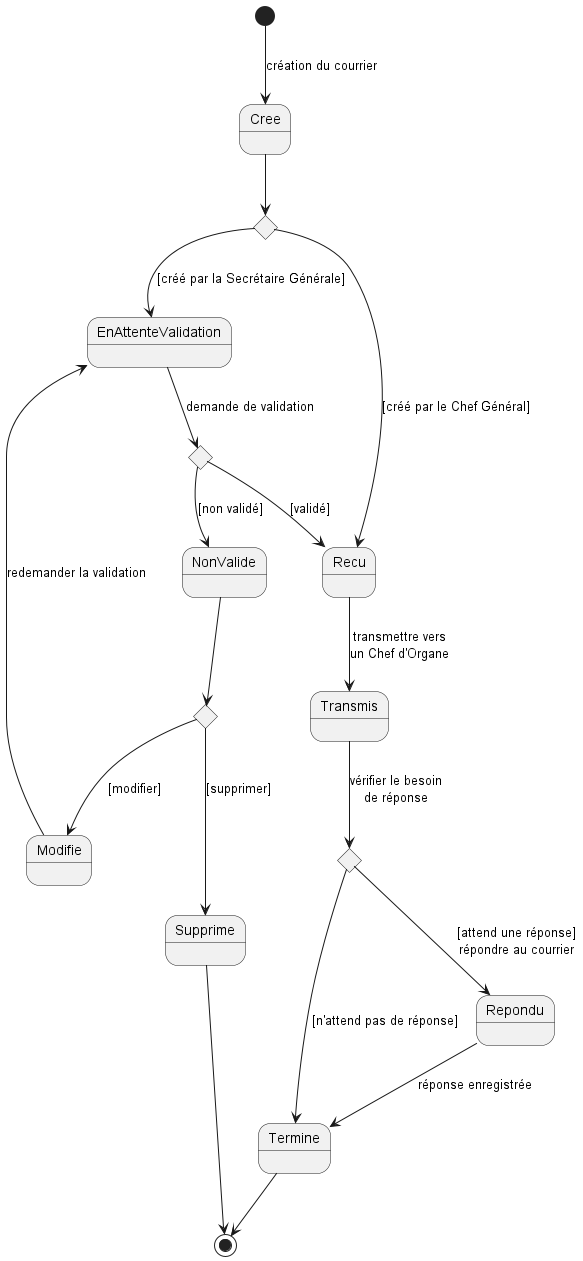
\includegraphics[width=\textwidth,height=0.85\textheight,keepaspectratio]{out/diagrams/usecases/puml/etat_courrier_creation_validation/etat_courrier.png}
    \caption{Diagramme d’états-transitions d’un courrier}
    \label{fig:etats_transitions_courrier}
\end{figure}

\chapter{Réalisation et Implémentation}
\label{chap:implementation}


\section{Introduction}
\label{sec:introduction_implementation}

Après avoir présenté l’analyse et la conception de notre système, ce chapitre est consacré à la réalisation pratique de l’application. Il permet de montrer comment les besoins définis précédemment ont été transformés en une solution web fonctionnelle pour la gestion du courrier.

Dans cette partie, nous présentons d’abord les outils et technologies utilisés durant le développement, notamment Laravel pour la partie serveur, React pour l’interface utilisateur, ainsi que les autres bibliothèques et services nécessaires au bon fonctionnement de l’application. Ensuite, nous expliquons le principe de communication entre le front-end et le back-end à travers une API REST, avant de donner un aperçu des principales interfaces réalisées.

Ce chapitre permet donc de passer de la conception théorique à l’implémentation réelle du système, en mettant en évidence les choix techniques adoptés et leur rôle dans le fonctionnement global de l’application.
\section{Environnement et outils de développement}
Le développement de notre application repose sur plusieurs outils utilisés pour gérer le serveur, l’interface, la base de données, la communication et la conception du système.

\subsection{Laravel}
\label{subsec:laravel}

\begin{figure}[H]
    \centering
    % Image à ajouter : logo officiel de Laravel
    % Exemple : images/laravel_logo.png
    
\includegraphics[width=0.25\textwidth]{images/logos/laravel.png}
    \caption{Logo du framework Laravel}
    \label{fig:laravel_logo}
\end{figure}

Laravel est un framework PHP utilisé dans notre projet pour gérer la logique de l’application, les routes, les contrôleurs, les modèles et les échanges avec la base de données. D’après la documentation officielle, Laravel est présenté comme un framework destiné au développement d’applications web en PHP \cite{laravel}. Il ne se limite pas seulement à l’écriture du code serveur, car il propose aussi plusieurs outils autour du développement, comme l’authentification, les notifications, les files d’attente, les migrations, Eloquent ORM, Sanctum et Reverb \cite{laraveldocs}. C’est pour cette raison que Laravel peut être considéré comme un écosystème complet. Dans notre application, il nous a surtout permis de créer une API RESTful, utilisée par l’interface React pour envoyer des requêtes, récupérer les données et effectuer les différentes opérations liées à la gestion du courrier.
\subsubsection{Eloquent ORM}
\label{subsubsec:eloquent_orm}

Eloquent ORM est l’outil de Laravel qui permet de travailler avec la base de données d’une manière plus simple. Au lieu d’écrire directement des requêtes SQL dans tout le projet, on utilise des classes appelées \textit{models}. Chaque modèle représente généralement une table de la base de données. Par exemple, dans notre application, un modèle \texttt{Courrier} peut représenter la table des courriers, tandis qu’un modèle \texttt{User} représente les utilisateurs du système. D’après la documentation officielle de Laravel, Eloquent associe chaque table de la base à un modèle qui permet de récupérer, ajouter, modifier ou supprimer les enregistrements \cite{laravel_eloquent}.

Dans notre projet, Eloquent nous a aidés à organiser la partie liée aux données. Les courriers, les utilisateurs, les pièces jointes, les commentaires et les messages peuvent être manipulés à partir de modèles. Cela rend le code plus lisible, surtout lorsque plusieurs opérations doivent être faites sur les mêmes données. Par exemple, au lieu d’écrire une requête SQL pour chercher les courriers reçus, on peut utiliser une méthode du modèle \texttt{Courrier}.

\begin{lstlisting}[language=PHP, caption={Exemple simple de modèle Eloquent}]
class Courrier extends Model
{
    protected $fillable = [
        'objet',
        'type',
        'statut',
        'priorite',
        'user_id',
        'structure_id'
    ];
}
\end{lstlisting}

Un autre point important dans Eloquent est la gestion des relations entre les tables. Dans une application de gestion de courrier, un courrier peut appartenir à un utilisateur, avoir plusieurs pièces jointes ou recevoir plusieurs commentaires. Ces relations peuvent être écrites directement dans les modèles. La documentation Laravel précise que les relations Eloquent sont définies comme des méthodes dans les classes des modèles, ce qui permet ensuite de les utiliser facilement dans les requêtes \cite{laravel_relationships}.

\begin{lstlisting}[language=PHP, caption={Exemple de relations dans un modèle Courrier}]
class Courrier extends Model
{
    public function utilisateur()
    {
        return $this->belongsTo(User::class, 'user_id');
    }

    public function piecesJointes()
    {
        return $this->hasMany(CourrierAttachment::class);
    }

    public function commentaires()
    {
        return $this->hasMany(CourrierComment::class);
    }
}
\end{lstlisting}

Les \textit{scopes} sont aussi très utiles dans Eloquent. Ils permettent de regrouper des conditions de recherche que l’on utilise souvent. Par exemple, dans notre application, on peut avoir besoin d’afficher seulement les courriers reçus, les courriers archivés ou les courriers en attente de validation. Au lieu de répéter les mêmes conditions dans plusieurs contrôleurs, on peut les mettre une seule fois dans le modèle. Laravel distingue notamment les scopes locaux et les scopes globaux. Les scopes locaux servent à réutiliser une condition précise dans certaines requêtes, alors que les scopes globaux s’appliquent automatiquement à toutes les requêtes d’un modèle \cite{laravel_eloquent}.

\begin{lstlisting}[language=PHP, caption={Exemple de scopes locaux pour les courriers}]
class Courrier extends Model
{
    public function scopeRecus($query)
    {
        return $query->where('type', 'recu');
    }

    public function scopeArchives($query)
    {
        return $query->where('statut', 'archive');
    }

    public function scopeEnAttente($query)
    {
        return $query->where('statut', 'en_attente');
    }
}
\end{lstlisting}

Après la définition de ces scopes, leur utilisation devient plus claire dans le contrôleur :

\begin{lstlisting}[language=PHP, caption={Utilisation des scopes dans un contrôleur}]
$courriersRecus = Courrier::recus()->get();

$courriersArchives = Courrier::archives()
    ->where('structure_id', $structureId)
    ->get();

$courriersEnAttente = Courrier::enAttente()->get();
\end{lstlisting}

Eloquent propose aussi d’autres fonctionnalités pratiques, comme les migrations, les timestamps automatiques, la suppression douce avec \texttt{SoftDeletes}, ainsi que les \textit{casts}. Les casts permettent de transformer automatiquement certains champs lorsqu’ils sont lus ou enregistrés. Par exemple, un champ de type date peut être manipulé directement comme un objet date, et un champ JSON peut être converti automatiquement en tableau PHP. La documentation officielle indique que les accessors, mutators et casts permettent de transformer les valeurs des attributs lorsqu’elles sont récupérées ou définies dans un modèle \cite{laravel_mutators}.

Dans notre application, Eloquent a donc joué un rôle important dans la communication avec la base de données. Il a permis de garder un code plus propre, de limiter la répétition des requêtes et de mieux représenter les éléments principaux du système sous forme de modèles liés entre eux.

\subsubsection{Laravel Sanctum}
\label{subsubsec:sanctum}
Laravel Sanctum est un package officiel de Laravel consacré à l’authentification. Il permet de sécuriser les applications de type SPA, les applications mobiles ainsi que les API simples basées sur des tokens \cite{laravel_sanctum}. Son rôle est de vérifier l’identité de l’utilisateur avant de lui donner accès aux ressources protégées. Il peut fonctionner soit avec les cookies de session, soit avec des tokens d’API envoyés avec les requêtes. Sanctum reste donc une solution assez simple à mettre en place, sans passer par un système plus lourd comme OAuth.

\subsubsection{Laravel Reverb}
\label{subsubsec:reverb}

\begin{figure}[H]
    \centering
    % Image à ajouter : logo officiel de Laravel Reverb
    % Exemple : images/reverb_logo.png
    
\includegraphics[width=0.25\textwidth]{images/logos/reverb_logo.png}
    \caption{Logo de Laravel Reverb}
    \label{fig:reverb_logo}
\end{figure}

Laravel Reverb est le serveur WebSocket officiel de Laravel. Il permet d’ajouter des échanges en temps réel dans une application, comme les notifications ou les messages instantanés. Reverb fonctionne avec le broadcasting de Laravel et reste compatible avec Laravel Echo grâce au protocole Pusher \cite{laravel_reverb}.
\subsection{React}
\label{subsec:react}

\begin{figure}[H]
    \centering
    % Image à ajouter : logo officiel de React
    % Exemple : images/react_logo.png
    
\includegraphics[width=0.22\textwidth]{images/logos/react_logo.png}
    \caption{Logo de React}
    \label{fig:react_logo}
\end{figure}

React est une bibliothèque JavaScript utilisée pour créer des interfaces utilisateur. Le site officiel la présente comme \textit{``the library for web and native user interfaces''} \cite{react}. Dans notre projet, React est utilisé pour construire les pages et les composants visibles par l’utilisateur.

\subsubsection{React Router DOM}
\label{subsubsec:react_router_dom}

React Router DOM permet de gérer la navigation entre les pages d’une application React. Il relie les URL aux composants affichés, ce qui permet de passer d’une page à une autre sans recharger toute l’application \cite{react_router}.

\subsubsection{Axios}
\label{subsubsec:axios}

\begin{figure}[H]
    \centering
    % Image à ajouter : logo officiel d'Axios
    % Exemple : images/axios_logo.png
    
\includegraphics[width=0.22\textwidth]{images/logos/axios_logo.png}
    \caption{Logo d’Axios}
    \label{fig:axios_logo}
\end{figure}

Axios est un client HTTP utilisé pour envoyer des requêtes vers une API. Sa documentation le définit comme un client HTTP simple pour le navigateur et Node.js \cite{axios}. Dans notre application, il sert surtout à envoyer les requêtes depuis React vers le serveur Laravel.
\subsection{Tailwind CSS}
\label{subsec:tailwind}
\begin{figure}[H]
    \centering
    % Image à ajouter : logo officiel de Tailwind CSS
    % Exemple : images/tailwind_logo.png
    
\includegraphics[width=0.22\textwidth]{images/logos/tailwind_logo.png}
    \caption{Logo de Tailwind CSS}
    \label{fig:tailwind_logo}
\end{figure}
Tailwind CSS est \textit{``a utility-first CSS framework for rapidly building modern websites without ever leaving your HTML''} \cite{tailwind}. Dans notre application, il sert surtout à styliser les composants React et à rendre l’interface plus claire, moderne et responsive.

\subsection{PlantUML}
\label{subsec:plantuml}

\begin{figure}[H]
    \centering
    % Image à ajouter : logo PlantUML
    % Exemple : images/plantuml_logo.png
    
\includegraphics[width=0.22\textwidth]{images/logos/plantuml_logo.png}
    \caption{Logo de PlantUML}
    \label{fig:plantuml_logo}
\end{figure}

PlantUML est un composant qui permet de dessiner rapidement des diagrammes UML à l’aide d’un langage simple et intuitif \cite{plantuml}.
\subsection{XAMPP}
\label{subsec:xampp}

\begin{figure}[H]
    \centering
    % Image à ajouter : logo XAMPP
    
\includegraphics[width=0.20\textwidth]{images/logos/xampp_logo.png}
    \caption{Logo de XAMPP}
    \label{fig:xampp_logo}
\end{figure}

XAMPP est une distribution Apache facile à installer qui contient MariaDB, PHP et Perl \cite{xampp}.

\subsubsection{MariaDB / MySQL}
\label{subsubsec:mariadb_mysql}

\begin{figure}[H]
    \centering
    % Image à ajouter : logo MariaDB
    
\includegraphics[width=0.22\textwidth]{images/logos/mariadb_logo.png}
    \caption{Logo de MariaDB}
    \label{fig:mariadb_logo}
\end{figure}

MariaDB Server est un système de gestion de base de données relationnelle open source \cite{mariadb}.

\subsubsection{Apache Server}
\label{subsubsec:apache_server}

\begin{figure}[H]
    \centering
    % Image à ajouter : logo Apache
    
\includegraphics[width=0.22\textwidth]{images/logos/apache_logo.png}
    \caption{Logo d'Apache HTTP Server}
    \label{fig:apache_logo}
\end{figure}

Apache HTTP Server est un serveur HTTP open source pour les systèmes d’exploitation modernes, y compris UNIX et Windows \cite{apache}.

\subsection{OCR}
\label{subsec:ocr}

\begin{figure}[H]
    \centering
    % Image à ajouter : logo Tesseract OCR
    
\includegraphics[width=0.22\textwidth]{images/logos/tesseract_logo.png}
    \caption{Logo de Tesseract OCR}
    \label{fig:tesseract_logo}
\end{figure}

Tesseract est un moteur de reconnaissance de texte open source OCR, disponible sous licence Apache 2.0 \cite{tesseract}. Dans notre projet, nous avons utilisé \texttt{tesseract.exe} pour extraire le texte à partir des documents numérisés.

\section{API RESTful}
\label{sec:api_restful}

Une API REST est une interface de programmation d'application qui respecte les principes de conception du style d'architecture REST \cite{rest_api}.

\section{Cycle de traitement d’une requête Laravel}
\label{sec:cycle_requete_laravel}

Dans une application Laravel, le traitement commence lorsqu’une requête HTTP arrive vers l’application. Le fichier \texttt{index.php} est le point d’entrée de toutes les requêtes, puis Laravel charge l’application et transmet la requête vers le routeur \cite{laravel_lifecycle}. Dans notre projet, cette requête peut être envoyée depuis React avec Axios. Axios est un \textit{``Promise based HTTP client for the browser and node.js''} \cite{axios}. Il permet donc d’envoyer une demande vers un endpoint Laravel, par exemple pour récupérer la liste des courriers ou enregistrer un nouveau courrier.

\begin{figure}[H]
    \centering
    % Image à ajouter : schéma du cycle d’une requête Laravel
    % Exemple : images/laravel_request_cycle.png
    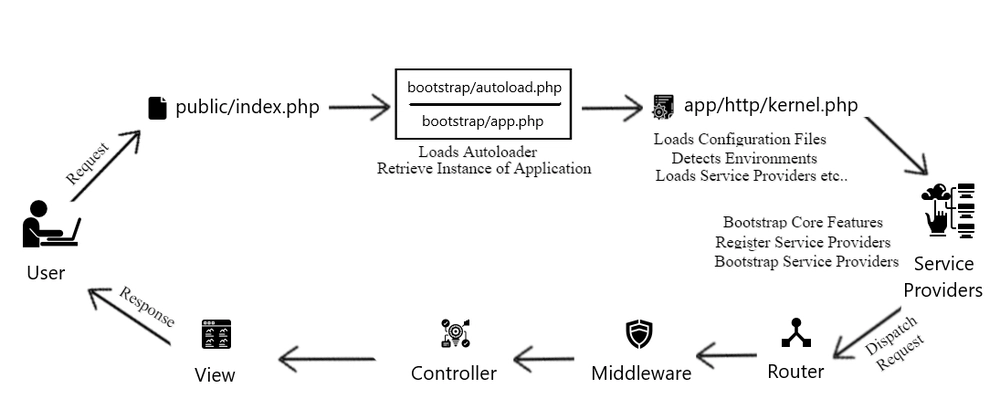
\includegraphics[width=0.85\textwidth]{images/logos/laravel_request_cycle.png }
    \caption{Cycle de traitement d’une requête Laravel\cite{patel_laravel_lifecycle}}
    \label{fig:laravel_request_cycle}
\end{figure}

Après l’arrivée de la requête, Laravel cherche la route correspondante, applique les middlewares nécessaires, puis exécute le contrôleur associé. La validation peut intervenir avant le traitement pour vérifier les données envoyées par l’utilisateur. Ensuite, le contrôleur utilise souvent un modèle Eloquent pour lire ou modifier les données dans la base. Une fois le traitement terminé, la réponse revient vers le client. Laravel précise que \textit{``All routes and controllers should return a response to be sent back to the user's browser''} \cite{laravel_responses}. Dans le cas d’une API, cette réponse est souvent envoyée au format JSON. JSON est un format textuel utilisé pour représenter des données structurées, ce qui le rend pratique pour transmettre les résultats vers le front-end \cite{mdn_json}. L’interface React peut ensuite exploiter ces données pour afficher les informations à l’utilisateur.
\section{Aperçu de l'application réalisée}
\label{sec:apercu_application}

Cette section présente ce qu’on voit dans l’application après avoir développé les pages principales. L’idée est de donner une première image de l’interface et des fonctionnalités, sans entrer dans le code.

\subsection{Tableau de bord}
\label{subsec:dashboard}

Le tableau de bord est la page d’accueil après connexion. On y trouve un résumé rapide des courriers et des notifications, pour savoir tout de suite si quelque chose demande une action.

\begin{figure}[H]
    \centering
    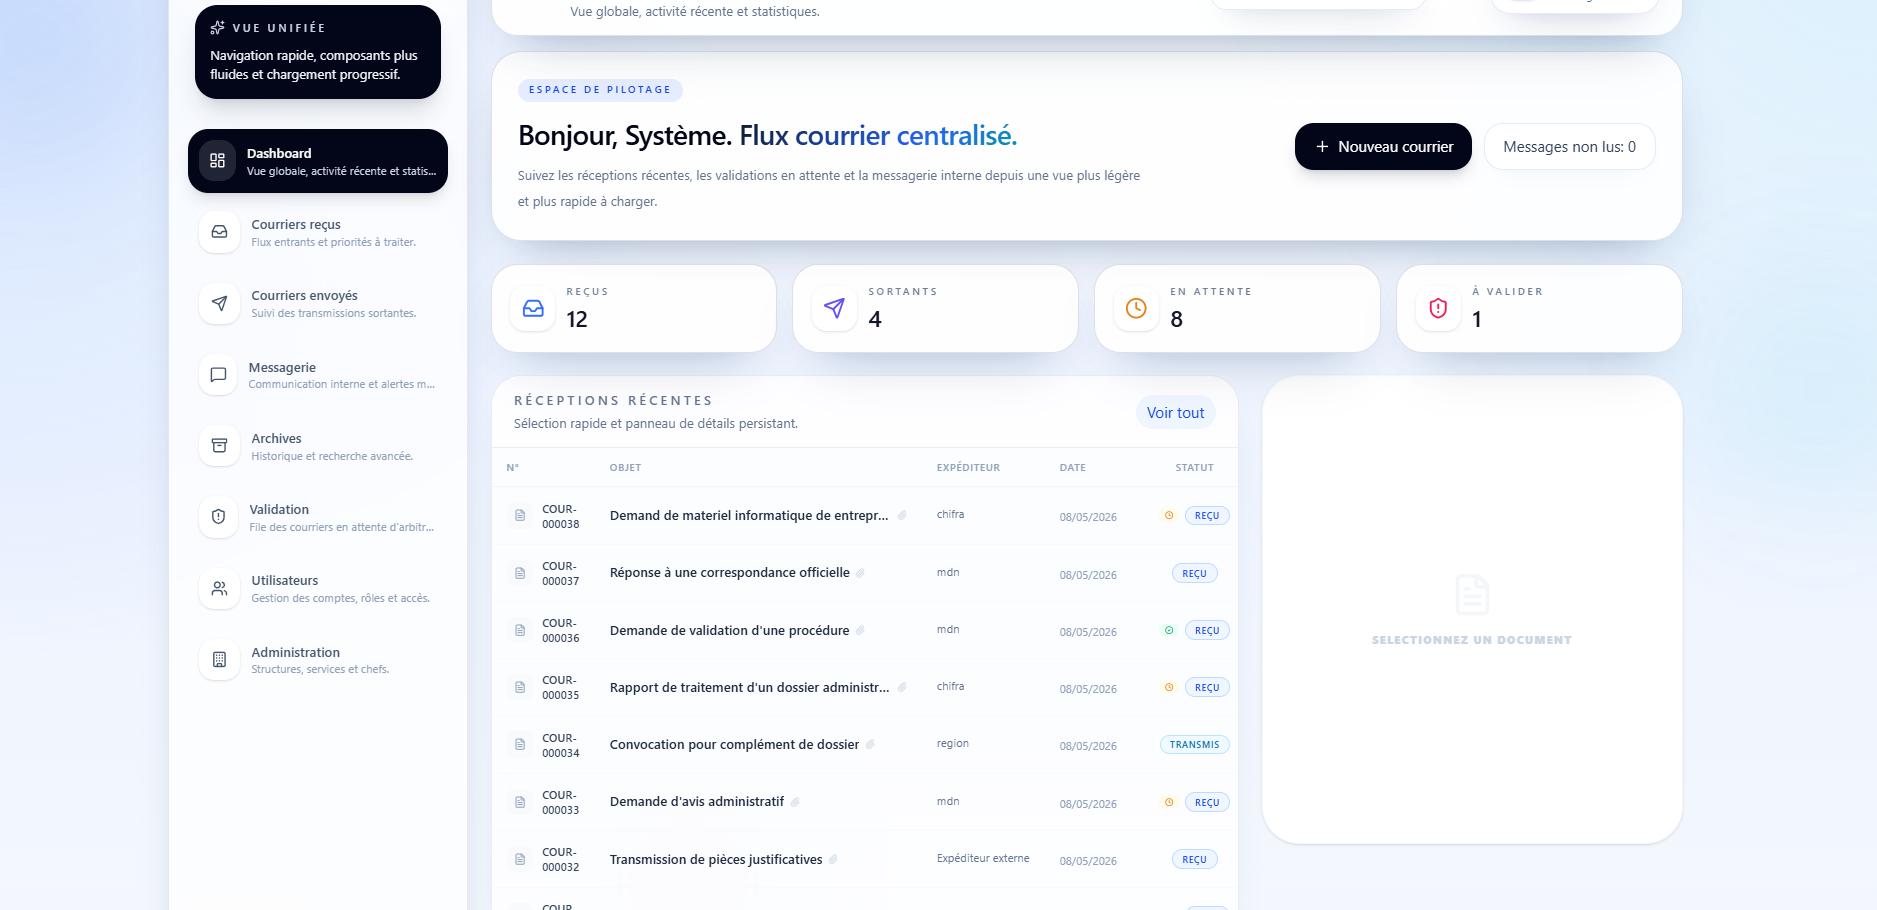
\includegraphics[width=0.92\textwidth,height=0.46\textheight,keepaspectratio]{images/app/dashboard.png}
    \caption{Vue du tableau de bord}
    \label{fig:dashboard_preview}
\end{figure}

\subsection{Gestion des courriers reçus}
\label{subsec:courriers_recus}

Cette partie du site regroupe tous les courriers entrants traités par l’application. L’utilisateur peut consulter la liste, filtrer et aller vers un courrier précis.

\begin{figure}[H]
    \centering
    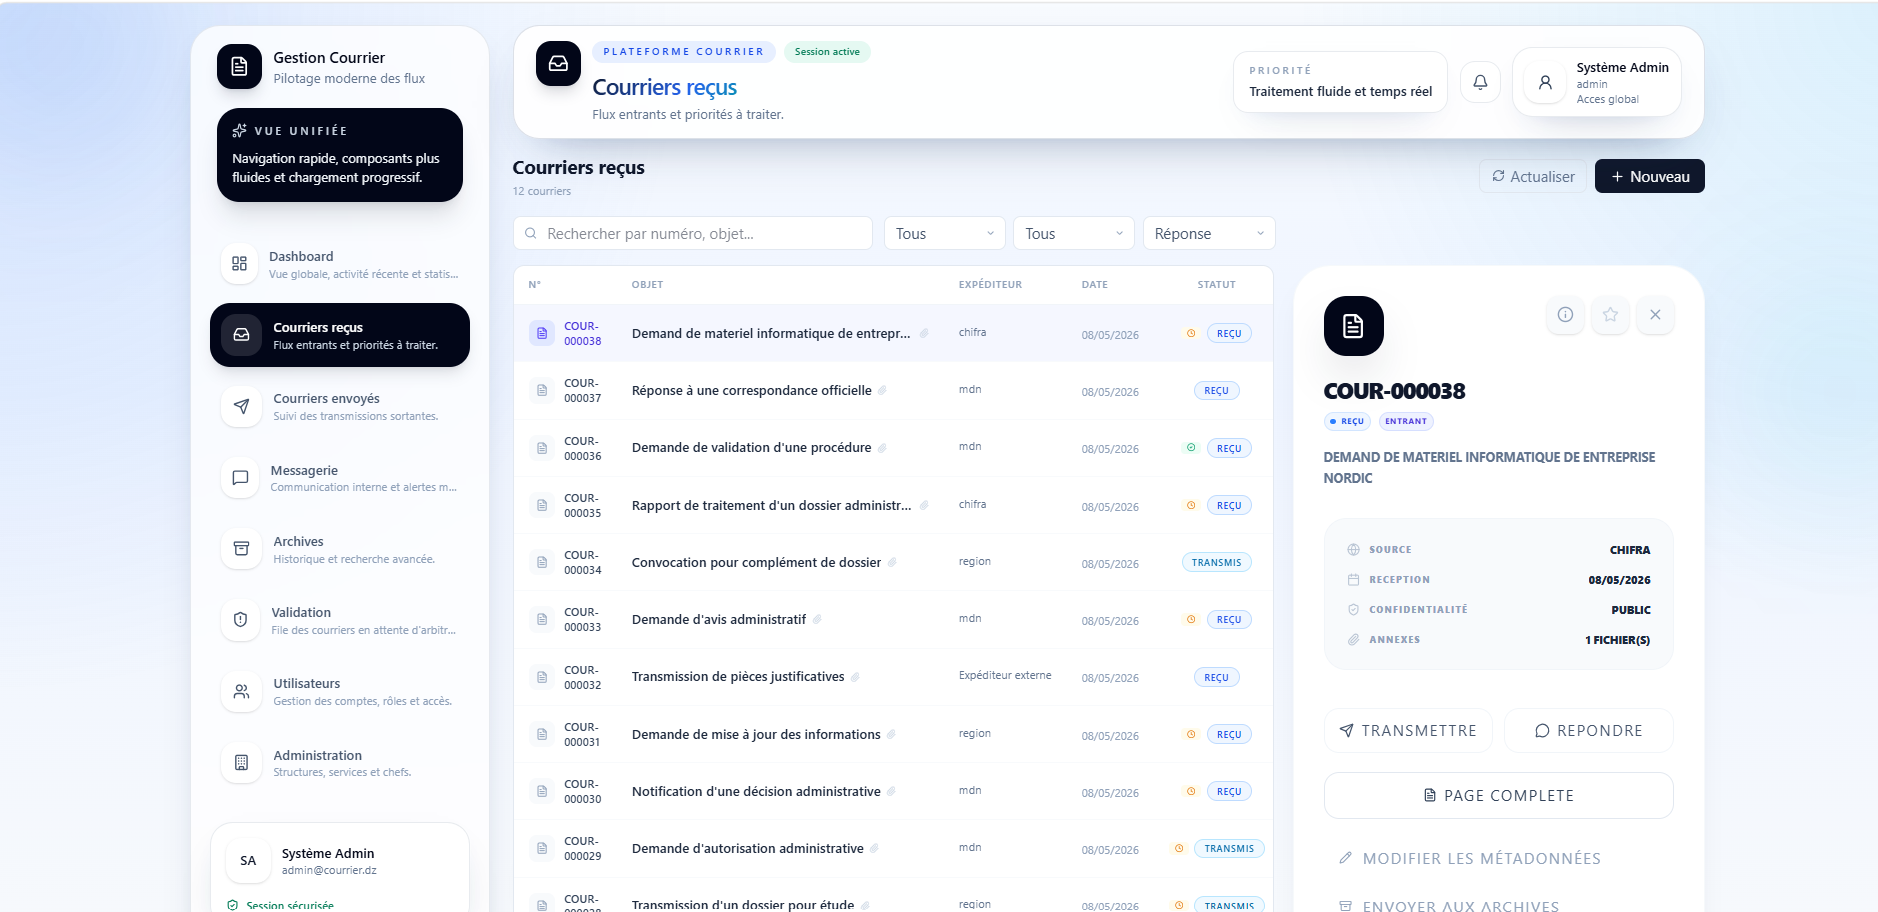
\includegraphics[width=0.92\textwidth,height=0.46\textheight,keepaspectratio]{images/app/courier_recu.png}
    \caption{Liste des courriers reçus}
    \label{fig:courriers_recus_list}
\end{figure}

\subsubsection{Création d’un nouveau courrier reçu}
\label{subsubsec:creation_courrier_recu}

La création d’un courrier reçu se fait avec un formulaire qui accepte l’objet, le service destinataire, la date et les pièces jointes. C’est la base pour entrer les documents qui arrivent dans l’organisation.

\begin{figure}[H]
    \centering
    \begin{minipage}{0.49\textwidth}
        \centering
        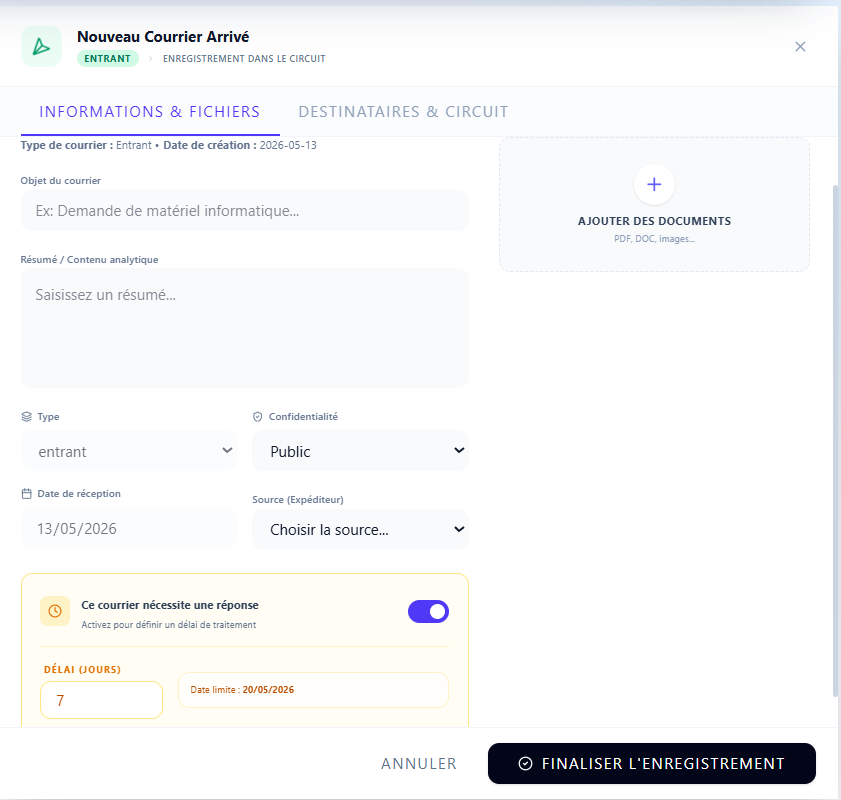
\includegraphics[width=\linewidth,height=0.36\textheight,keepaspectratio]{images/app/courier_recu_crre1.png}
    \end{minipage}
    \hfill
    \begin{minipage}{0.49\textwidth}
        \centering
        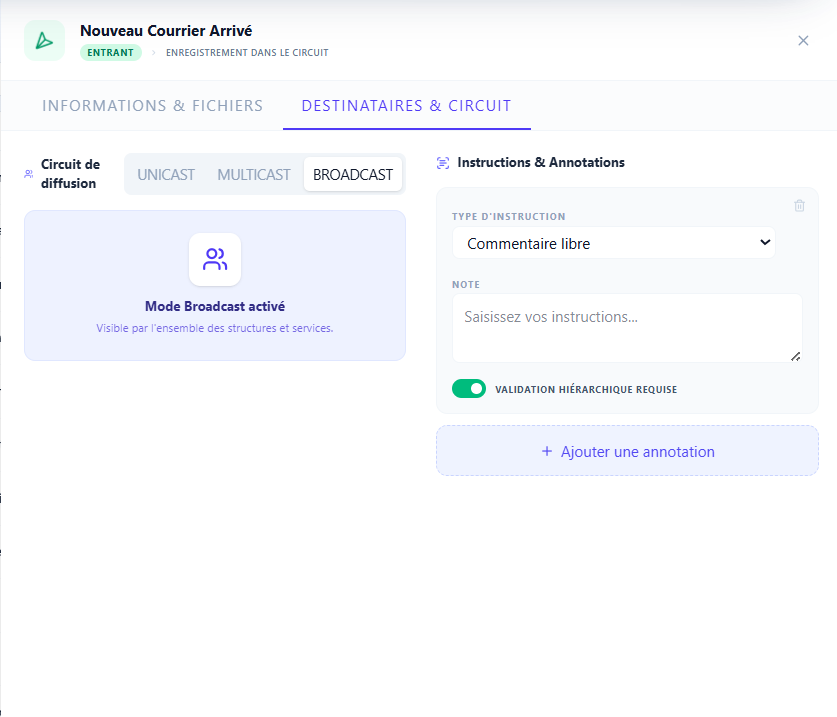
\includegraphics[width=\linewidth,height=0.36\textheight,keepaspectratio]{images/app/courier_recu_crr2.png}
    \end{minipage}
    \caption{Formulaire de création d’un courrier reçu}
    \label{fig:creation_courrier_recu}
\end{figure}

\subsubsection{Transmission d’un courrier}
\label{subsubsec:transmission_courrier}

Quand il faut transférer un courrier vers un autre service ou responsable, la transmission permet d’avancer le dossier. L’interface propose un bouton de transmission et un suivi d’état simple.

\begin{figure}[H]
    \centering
    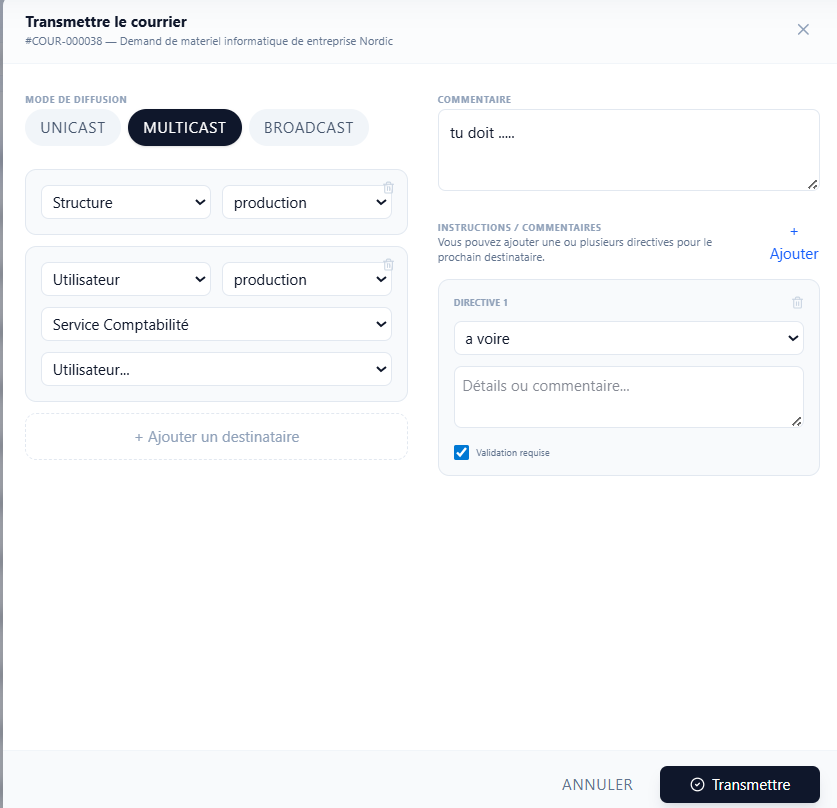
\includegraphics[width=0.90\textwidth,height=0.44\textheight,keepaspectratio]{images/app/trans.png}
    \caption{Écran de transmission d’un courrier}
    \label{fig:transmission_courrier}
\end{figure}

\subsubsection{Réponse à un courrier}
\label{subsubsec:reponse_courrier}

La réponse à un courrier s’effectue depuis le détail du courrier reçu, avec un formulaire pré-rempli et des destinataires suggérés selon le workflow.

\begin{figure}[H]
    \centering
    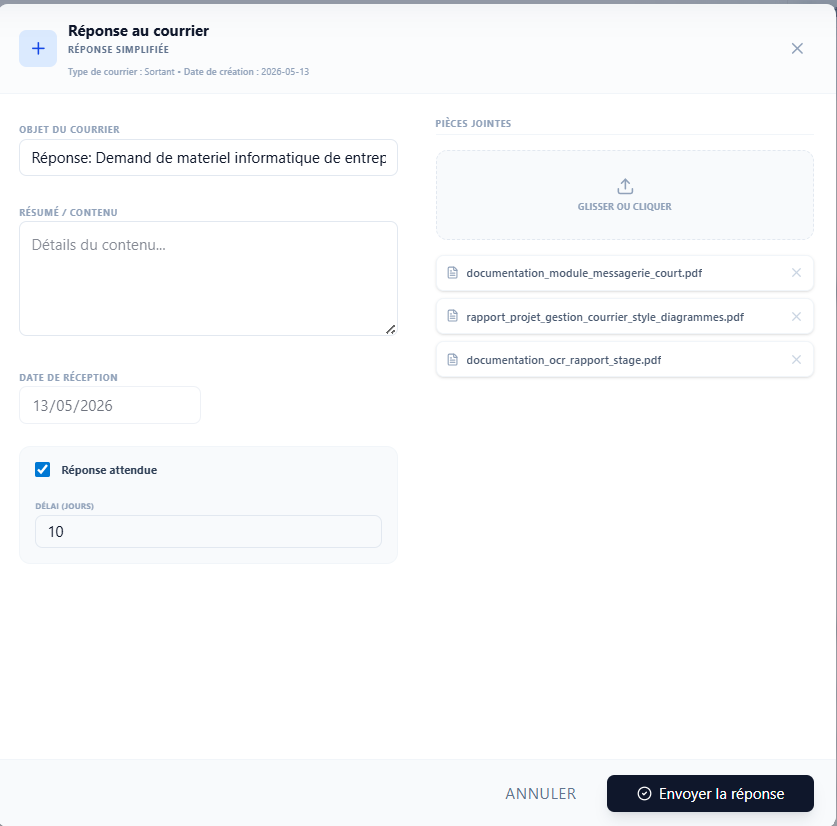
\includegraphics[width=0.90\textwidth,height=0.3\textheight,keepaspectratio]{images/app/respo_cor.png}
    \caption{Interface de réponse à un courrier}
    \label{fig:reponse_courrier}
\end{figure}

\subsubsection{Archivage d’un courrier}
\label{subsubsec:archivage_courrier}

L’archivage permet de ranger un courrier hors du flux actif, tout en le gardant accessible pour consultation future. Le système retire le courrier de la vue principale sans le supprimer.

\begin{figure}[H]
    \centering
    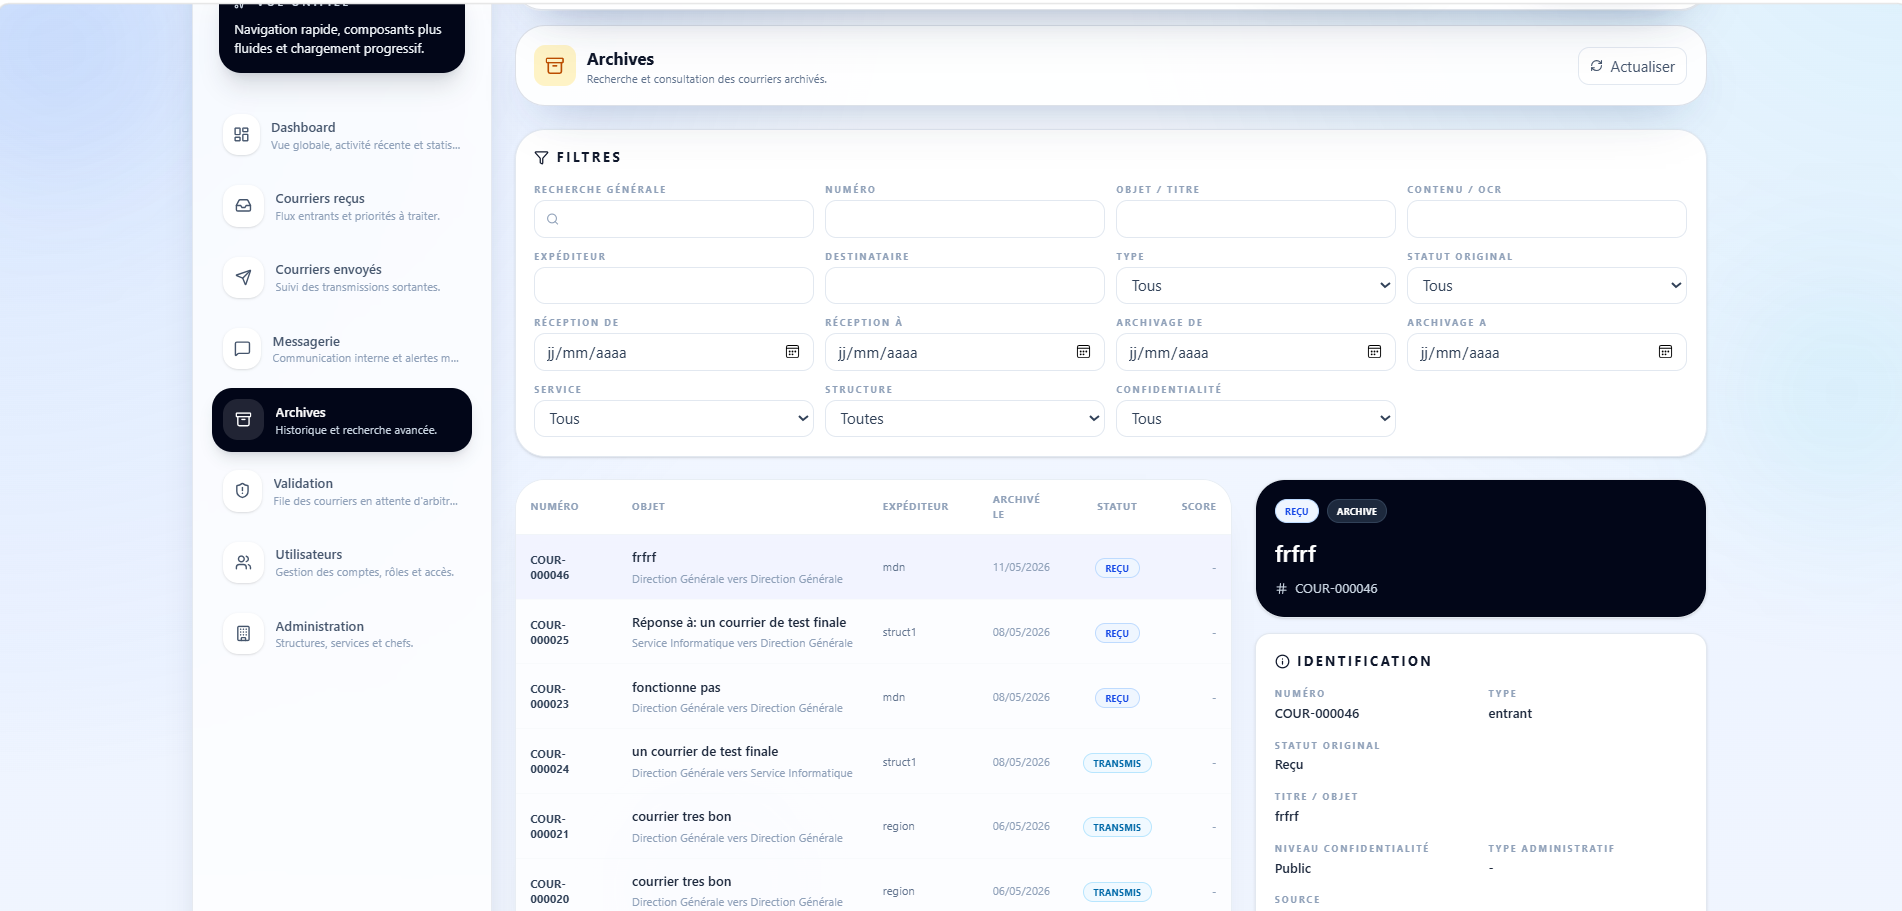
\includegraphics[width=0.90\textwidth,height=0.44\textheight,keepaspectratio]{images/app/archive.png}
    \caption{Archivage d’un courrier}
    \label{fig:archivage_courrier}
\end{figure}


\subsection{Gestion des courriers envoyés}
\label{subsec:courriers_envoyes}

Cette section liste les courriers sortants. Elle montre les envois déjà effectués, les brouillons et les éléments en attente de validation.

\begin{figure}[H]
    \centering
    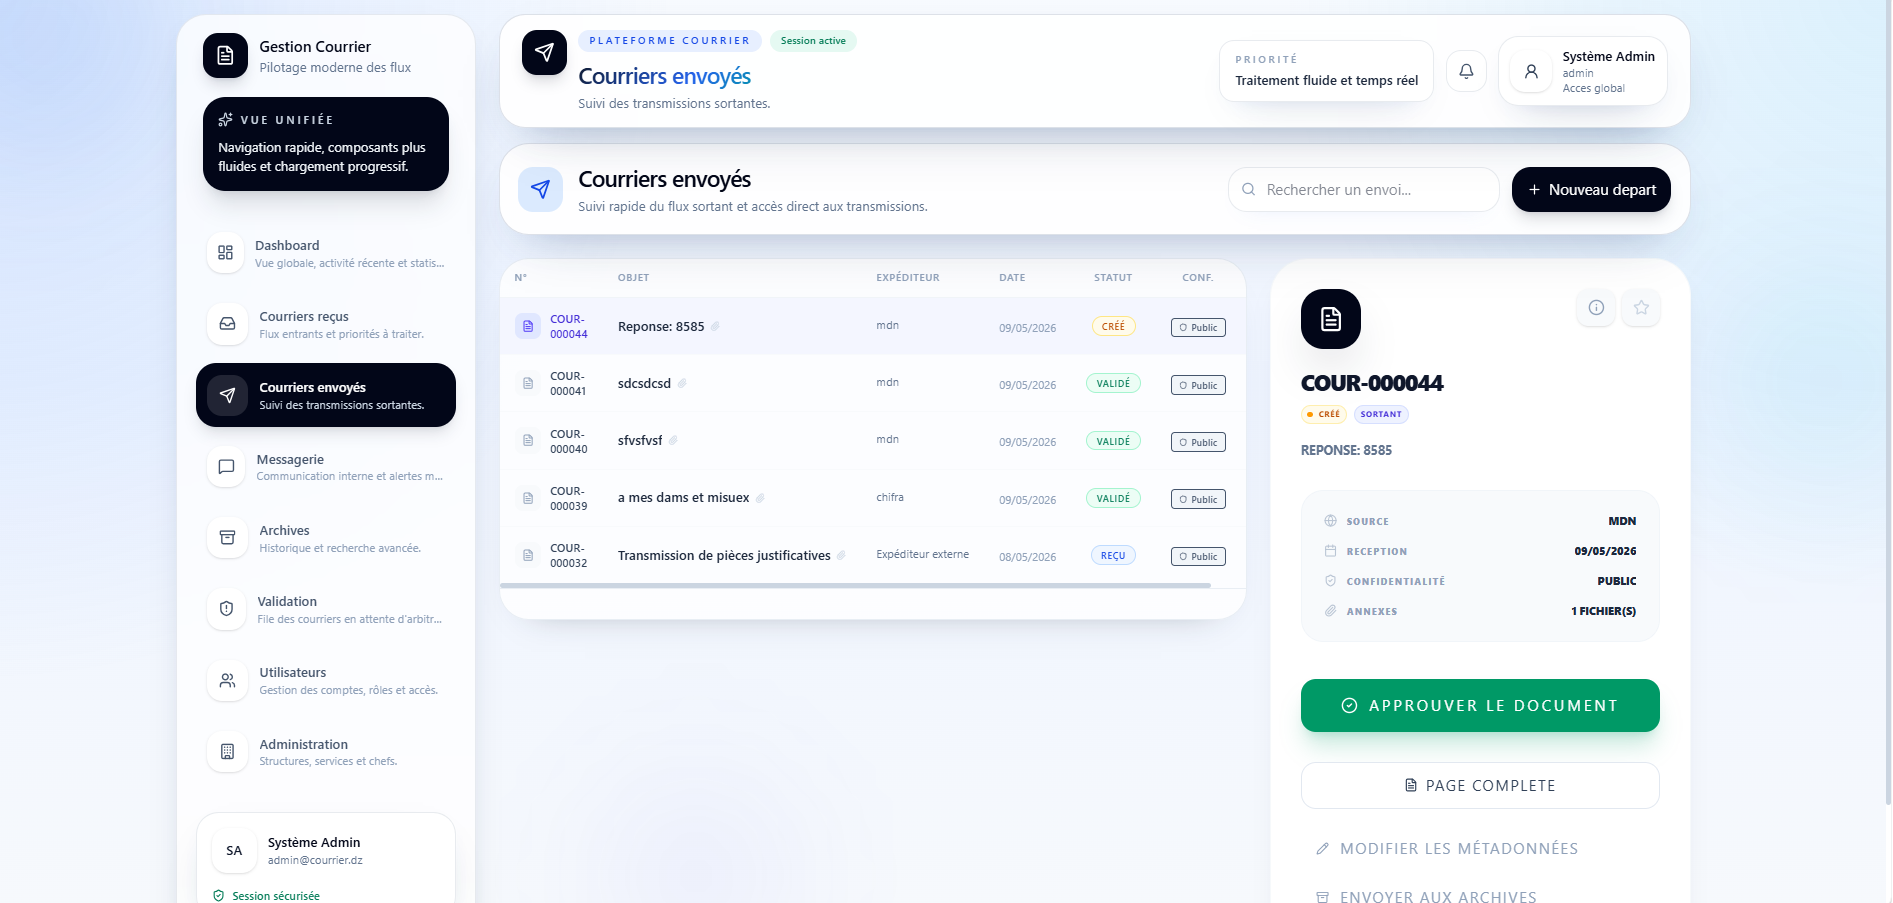
\includegraphics[width=0.92\textwidth,height=0.40\textheight,keepaspectratio]{images/app/courrier_env.png}
    \caption{Liste des courriers envoyés}
    \label{fig:courriers_envoyes}
\end{figure}

\subsubsection{Création d’un nouveau courrier envoyé}
\label{subsubsec:creation_courrier_envoye}

Le formulaire d’envoi permet de rédiger un courrier sortant, de choisir la confidentialité et les destinataires, puis de l’enregistrer ou de le soumettre.

\begin{figure}[H]
    \centering
    \begin{minipage}{0.49\textwidth}
        \centering
        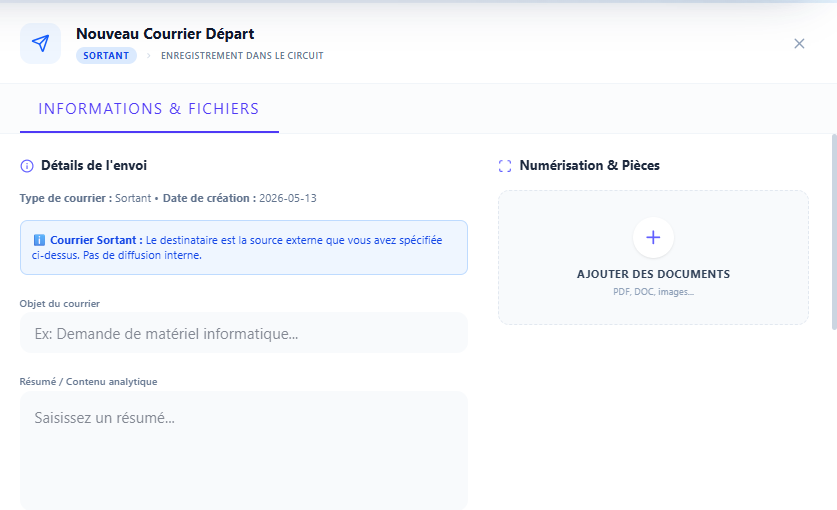
\includegraphics[width=\linewidth,height=0.36\textheight,keepaspectratio]{images/app/Courier_envoye_create.png}
    \end{minipage}
    \hfill
    \begin{minipage}{0.49\textwidth}
        \centering
        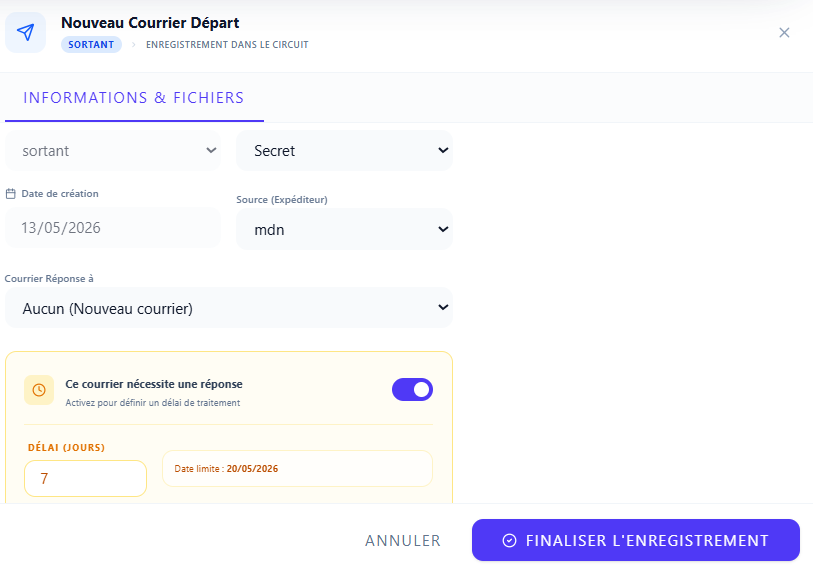
\includegraphics[width=\linewidth,height=0.36\textheight,keepaspectratio]{images/app/coureur_env_crea2.png}
    \end{minipage}
    \caption{Formulaire de création d’un courrier envoyé}
    \label{fig:creation_courrier_envoye}
\end{figure}

\subsection{Messagerie interne}
\label{subsec:messagerie_interne}

La messagerie interne sert à communiquer rapidement entre utilisateurs quand un courrier ne suffit pas. Elle permet d’envoyer et de recevoir des messages privés.

\begin{figure}[H]
    \centering
    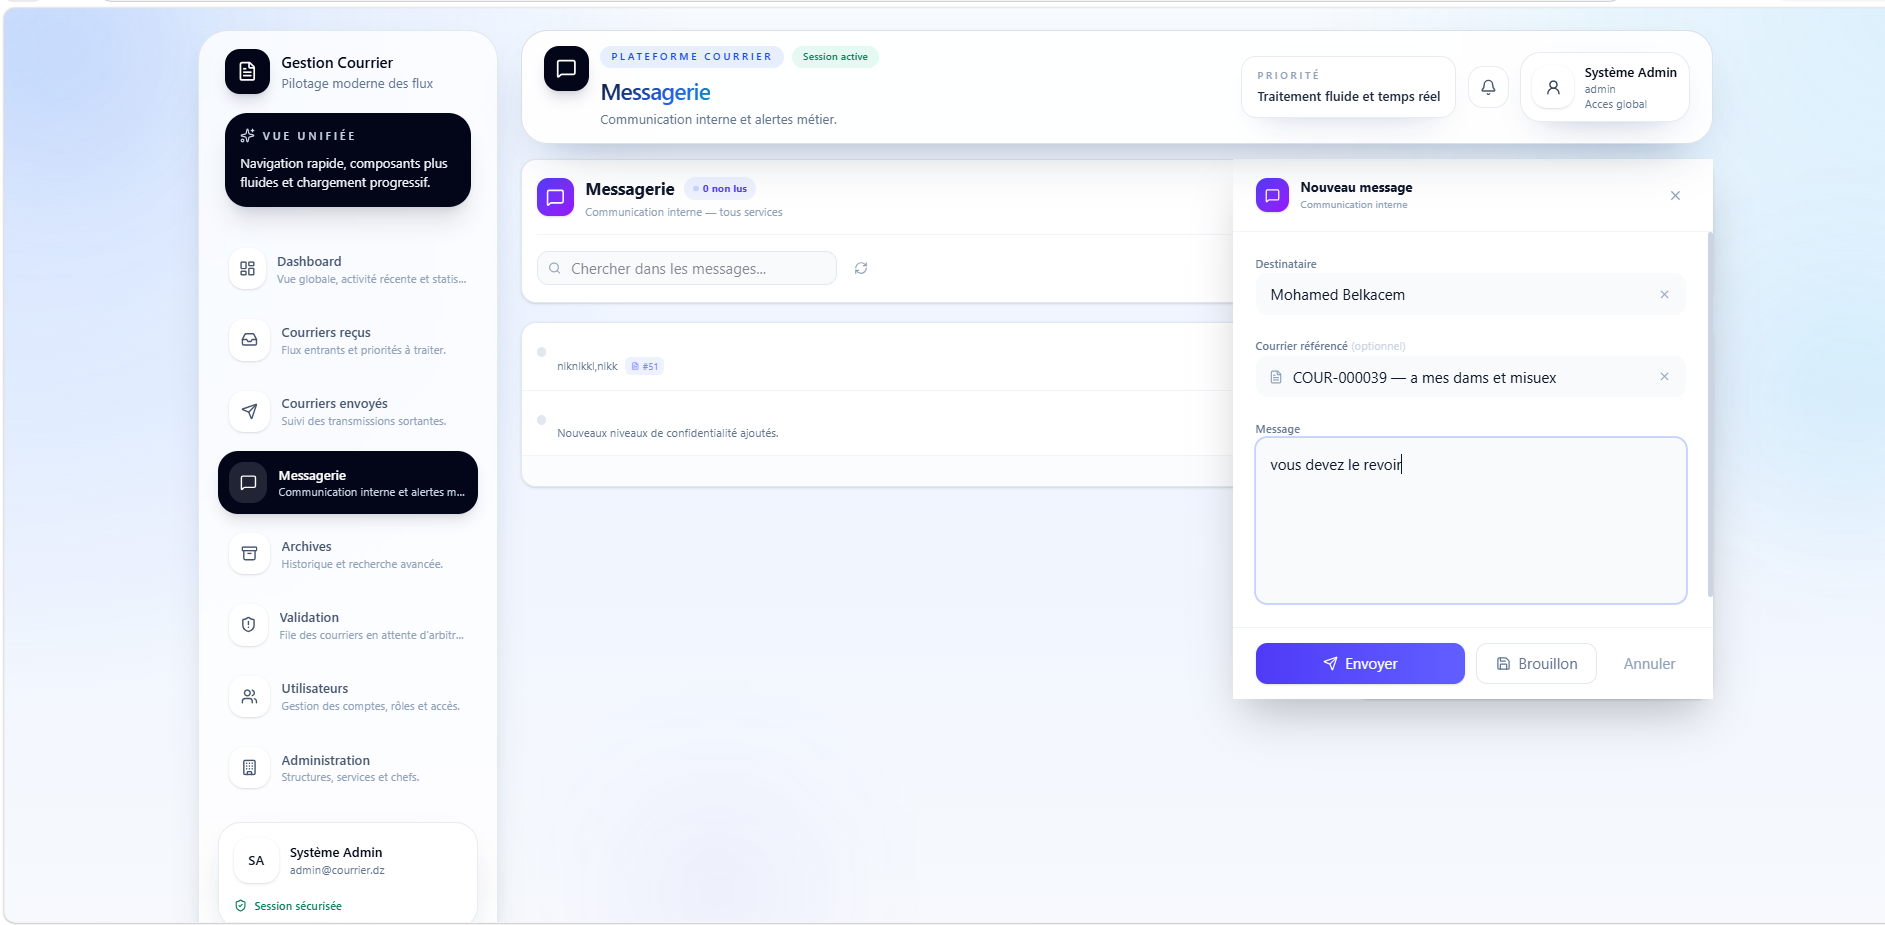
\includegraphics[width=0.90\textwidth,height=0.44\textheight,keepaspectratio]{images/app/msg_+create.png}
    \caption{Messagerie interne}
    \label{fig:messagerie_interne}
\end{figure}

\subsubsection{Création d’un nouveau message}
\label{subsubsec:creation_message}

L’utilisateur compose son message, choisit un destinataire et peut l’envoyer ou le sauvegarder en brouillon. C’est simple et direct.

\begin{figure}[H]
    \centering
    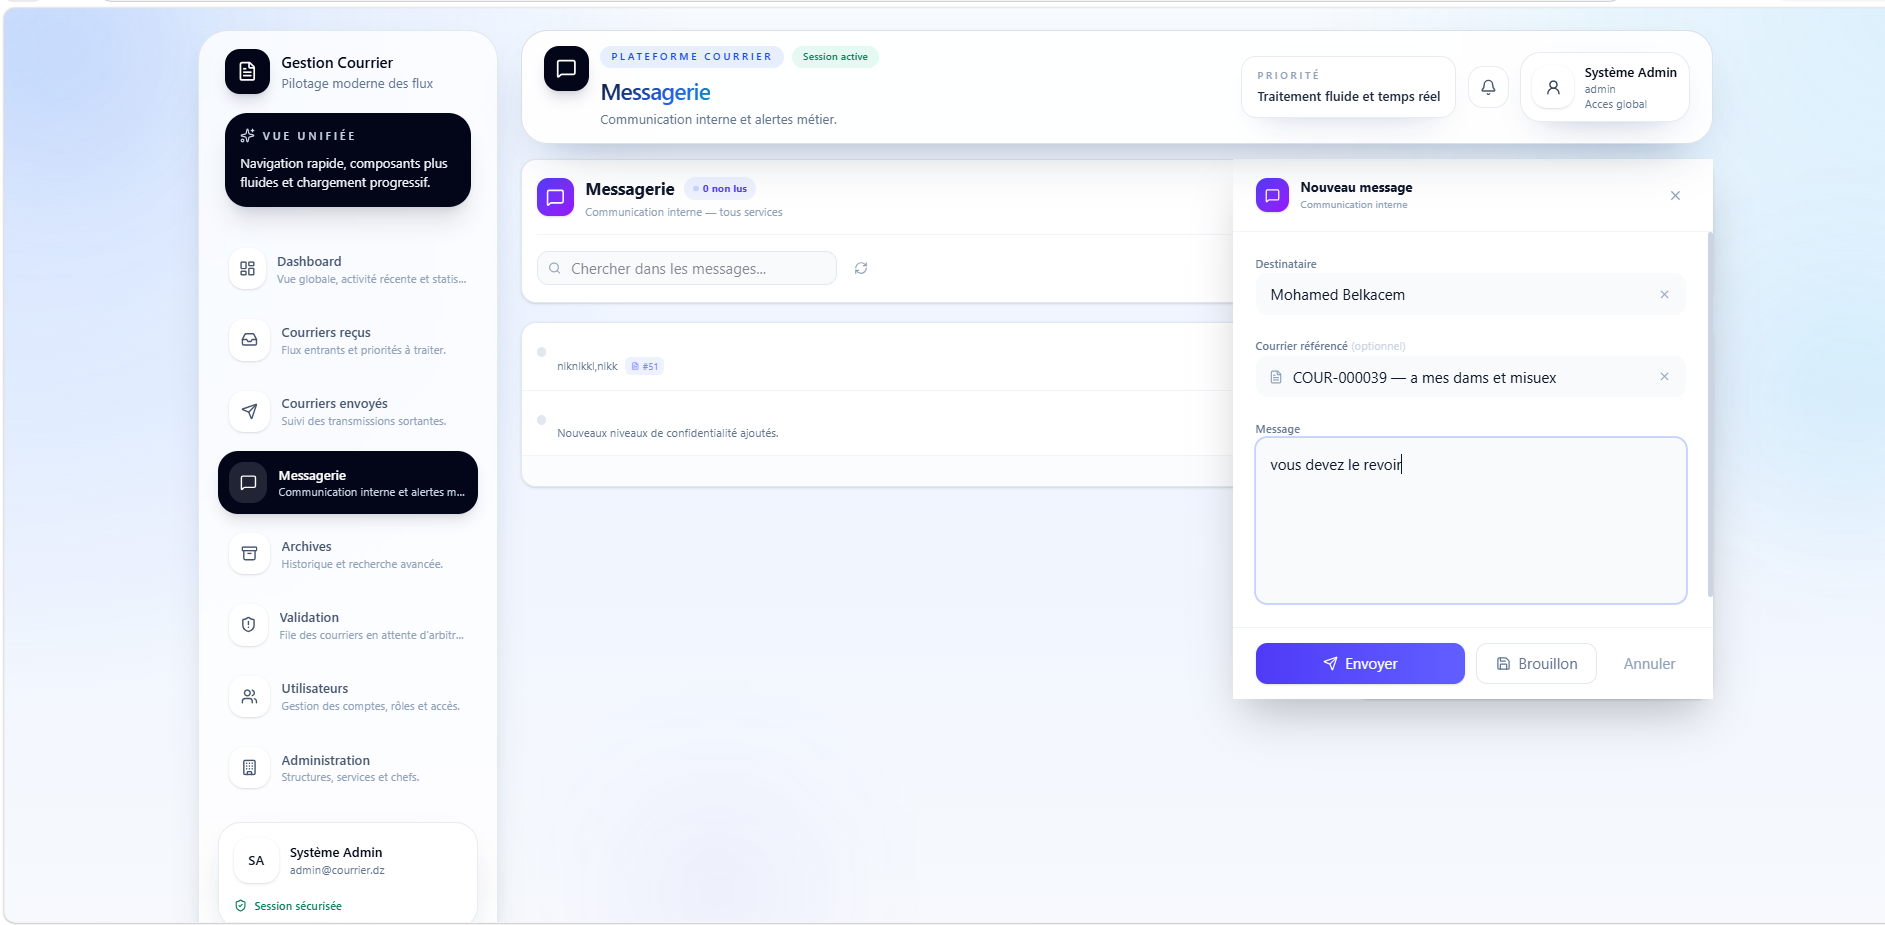
\includegraphics[width=0.90\textwidth,height=0.44\textheight,keepaspectratio]{images/app/msg_+create.png}
    \caption{Création d’un nouveau message}
    \label{fig:creation_message}
\end{figure}

\subsubsection{Consultation des messages}
\label{subsubsec:consultation_messages}

La consultation permet de lire les messages reçus et envoyés, avec le statut lu/non-lu et la possibilité de filtrer par destinataire.

\begin{figure}[H]
    \centering
    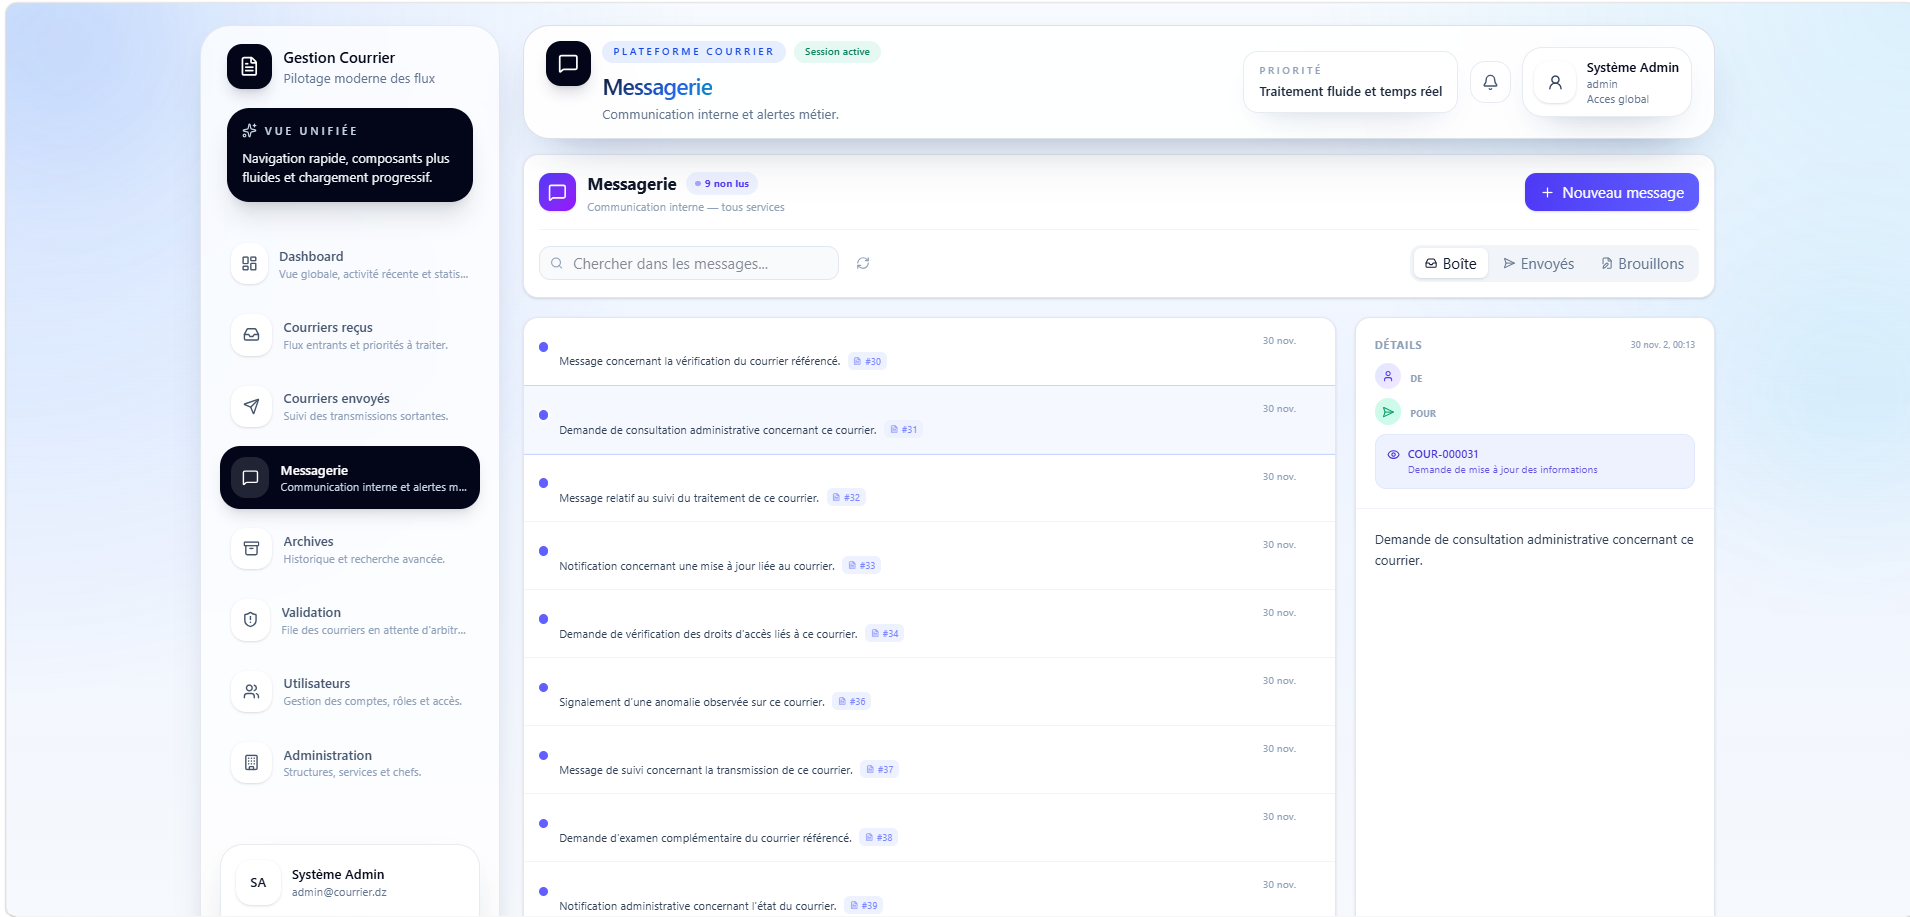
\includegraphics[width=0.90\textwidth,height=0.44\textheight,keepaspectratio]{images/app/cons_im.png}
    \caption{Consultation des messages}
    \label{fig:consultation_messages}
\end{figure}

\subsection{Gestion des archives}
\label{subsec:gestion_archives}

La gestion des archives permet de retrouver un courrier classé par le passé. C’est utile pour garder l’historique sans encombrer les listes actives.

\begin{figure}[H]
    \centering
    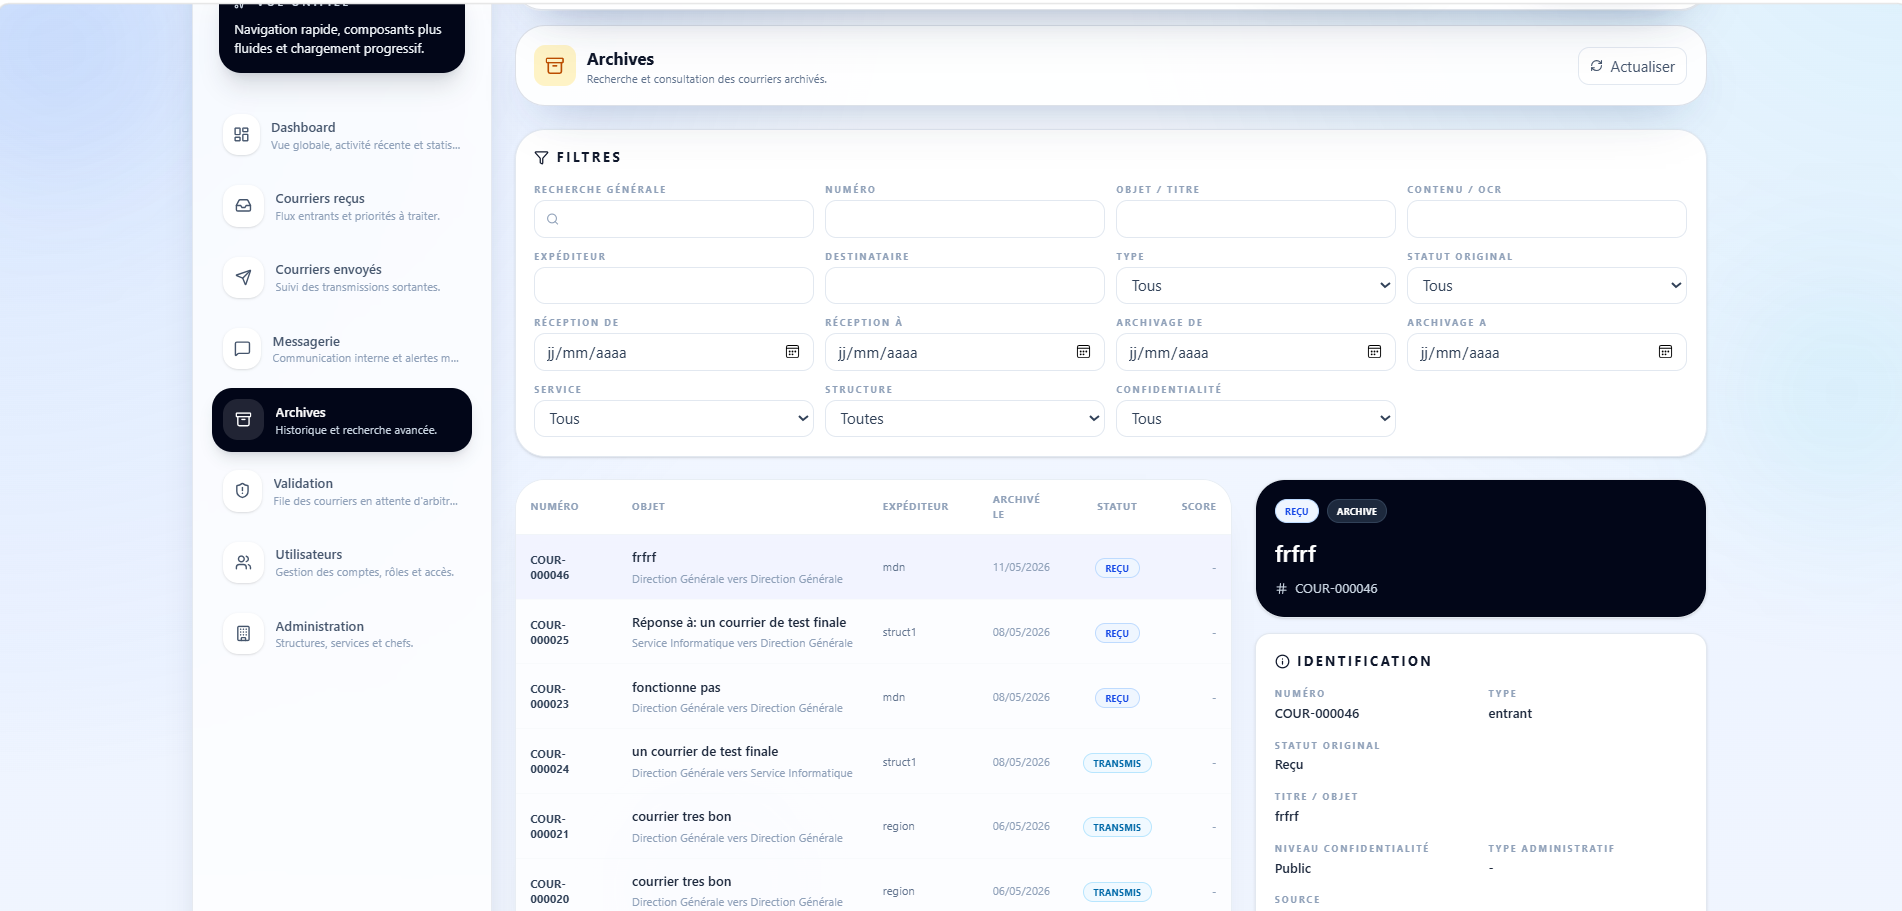
\includegraphics[width=0.90\textwidth,height=0.44\textheight,keepaspectratio]{images/app/archive.png}
    \caption{Vue de la gestion des archives}
    \label{fig:gestion_archives}
\end{figure}

\subsubsection{Recherche et filtrage des courriers archivés}
\label{subsubsec:recherche_filtre_archives}

Le moteur de recherche des archives accepte plusieurs critères : numéro, objet, date ou statut. Cela aide à retrouver rapidement un courrier ancien.

\begin{figure}[H]
    \centering
    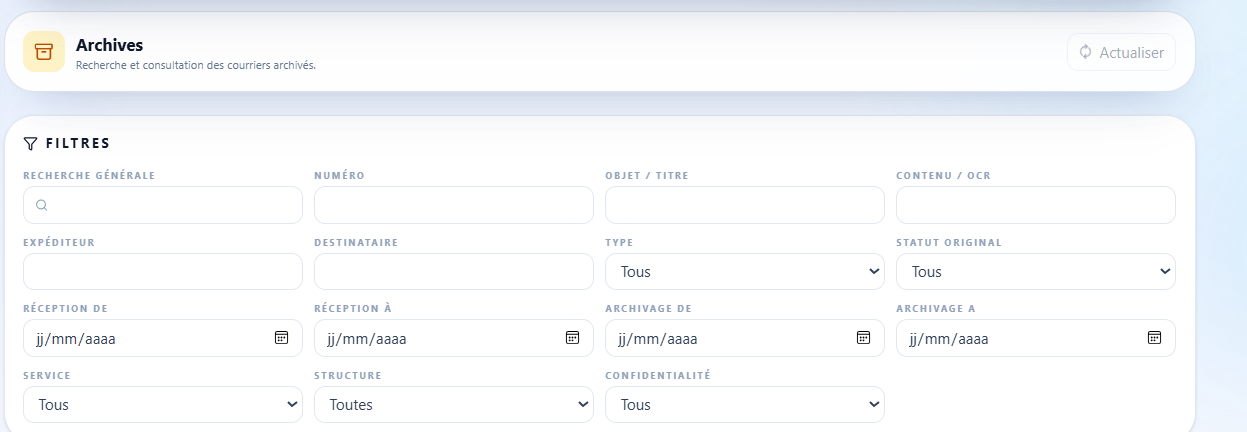
\includegraphics[width=0.90\textwidth,height=0.44\textheight,keepaspectratio]{images/app/filtre.png}
    \caption{Recherche et filtrage des archives}
    \label{fig:recherche_filtre_archives}
\end{figure}


\subsection{Gestion de l’administration}
\label{subsec:gestion_administration}

Cette partie est réservée à l’administrateur. Elle permet d’organiser les entités de l’application, notamment les structures, les services et l’affectation des responsables. Grâce à ces interfaces, l’administration peut préparer l’environnement de travail avant l’utilisation quotidienne du système par les autres profils.
\subsubsection{Gestion des utilisateurs}
\label{subsec:gestion_utilisateurs}

Cette page de gestion est destinée aux administrateurs. Elle affiche les profils utilisateurs, les rôles et les droits, et permet de modifier ou supprimer des comptes.

\begin{figure}[H]
    \centering
    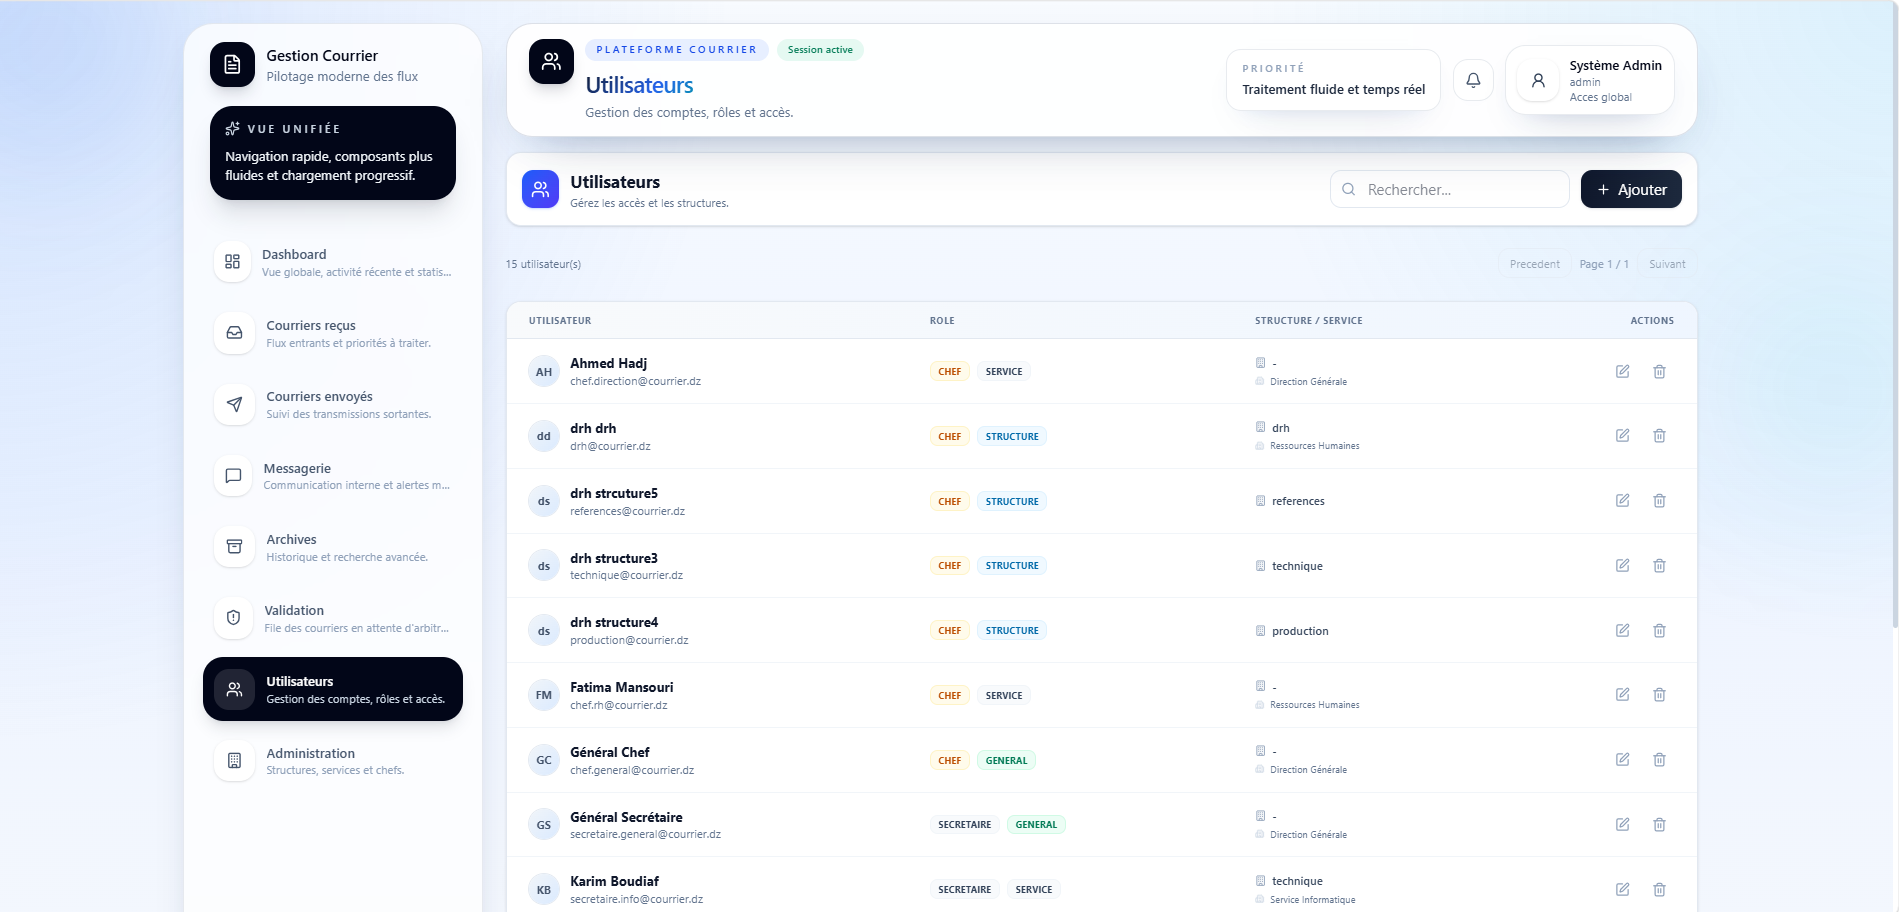
\includegraphics[width=0.90\textwidth,height=0.44\textheight,keepaspectratio]{images/app/users_index.png}
    \caption{Gestion des utilisateurs}
    \label{fig:gestion_utilisateurs}
\end{figure}

\subsubsection{Affichage des structures}
\label{subsubsec:affichage_structures}

L’affichage des structures permet à l’administrateur de consulter les différentes entités organisationnelles enregistrées dans l’application. Cette interface facilite le suivi des structures existantes et prépare les opérations d’ajout, de modification ou de suppression.

\begin{figure}[H]
    \centering
    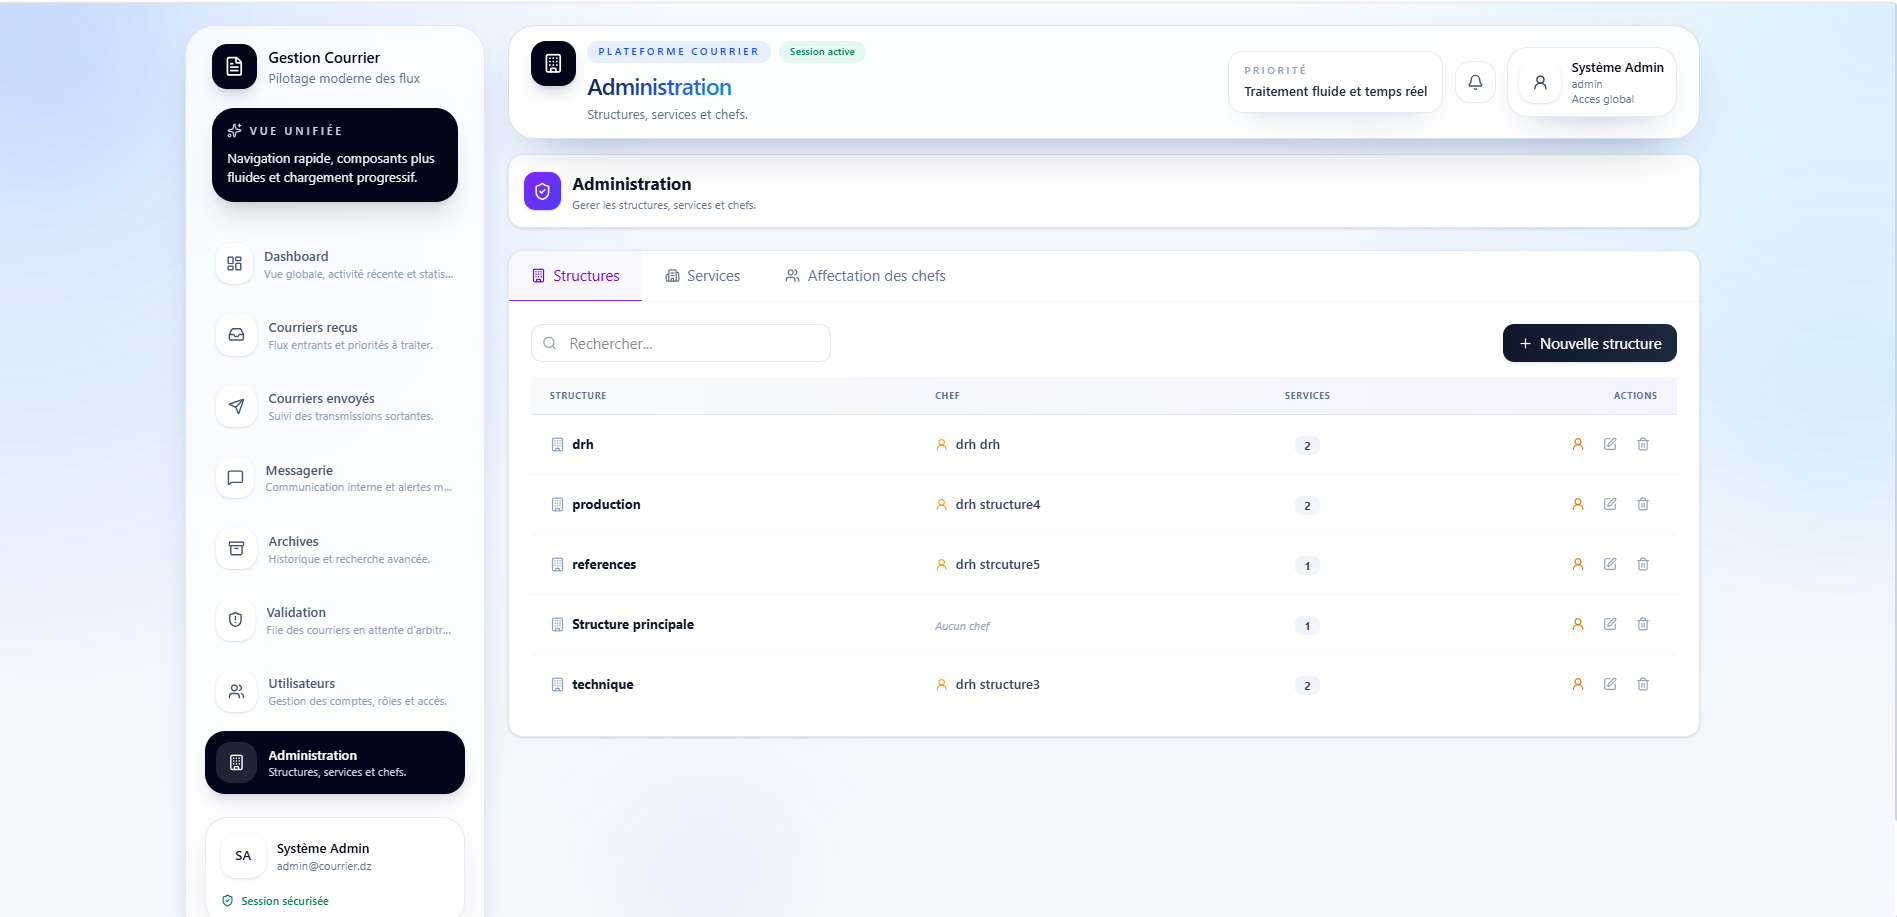
\includegraphics[width=0.92\textwidth,height=0.46\textheight,keepaspectratio]{images/app/adminstrationindex.png}
    \caption{Affichage des structures}
    \label{fig:affichage_structures}
\end{figure}

\subsubsection{Création d’une structure}
\label{subsubsec:creation_structure}

La création d’une structure permet d’ajouter une direction ou une entité organisationnelle dans le système. Cette structure pourra ensuite être utilisée pour rattacher des services et organiser les utilisateurs.

\begin{figure}[H]
    \centering
    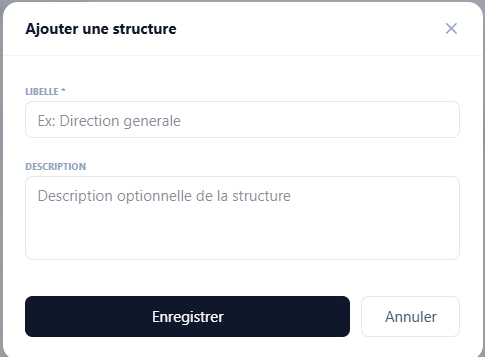
\includegraphics[width=0.88\textwidth,height=0.42\textheight,keepaspectratio]{images/app/struct_crr.png}
    \caption{Création d’une structure}
    \label{fig:creation_structure}
\end{figure}

\subsubsection{Affichage des services}
\label{subsubsec:affichage_services}

L’affichage des services présente la liste des services disponibles dans l’application. Chaque service est rattaché à une structure, ce qui permet de mieux organiser les utilisateurs et les circuits de traitement des courriers.

\begin{figure}[H]
    \centering
    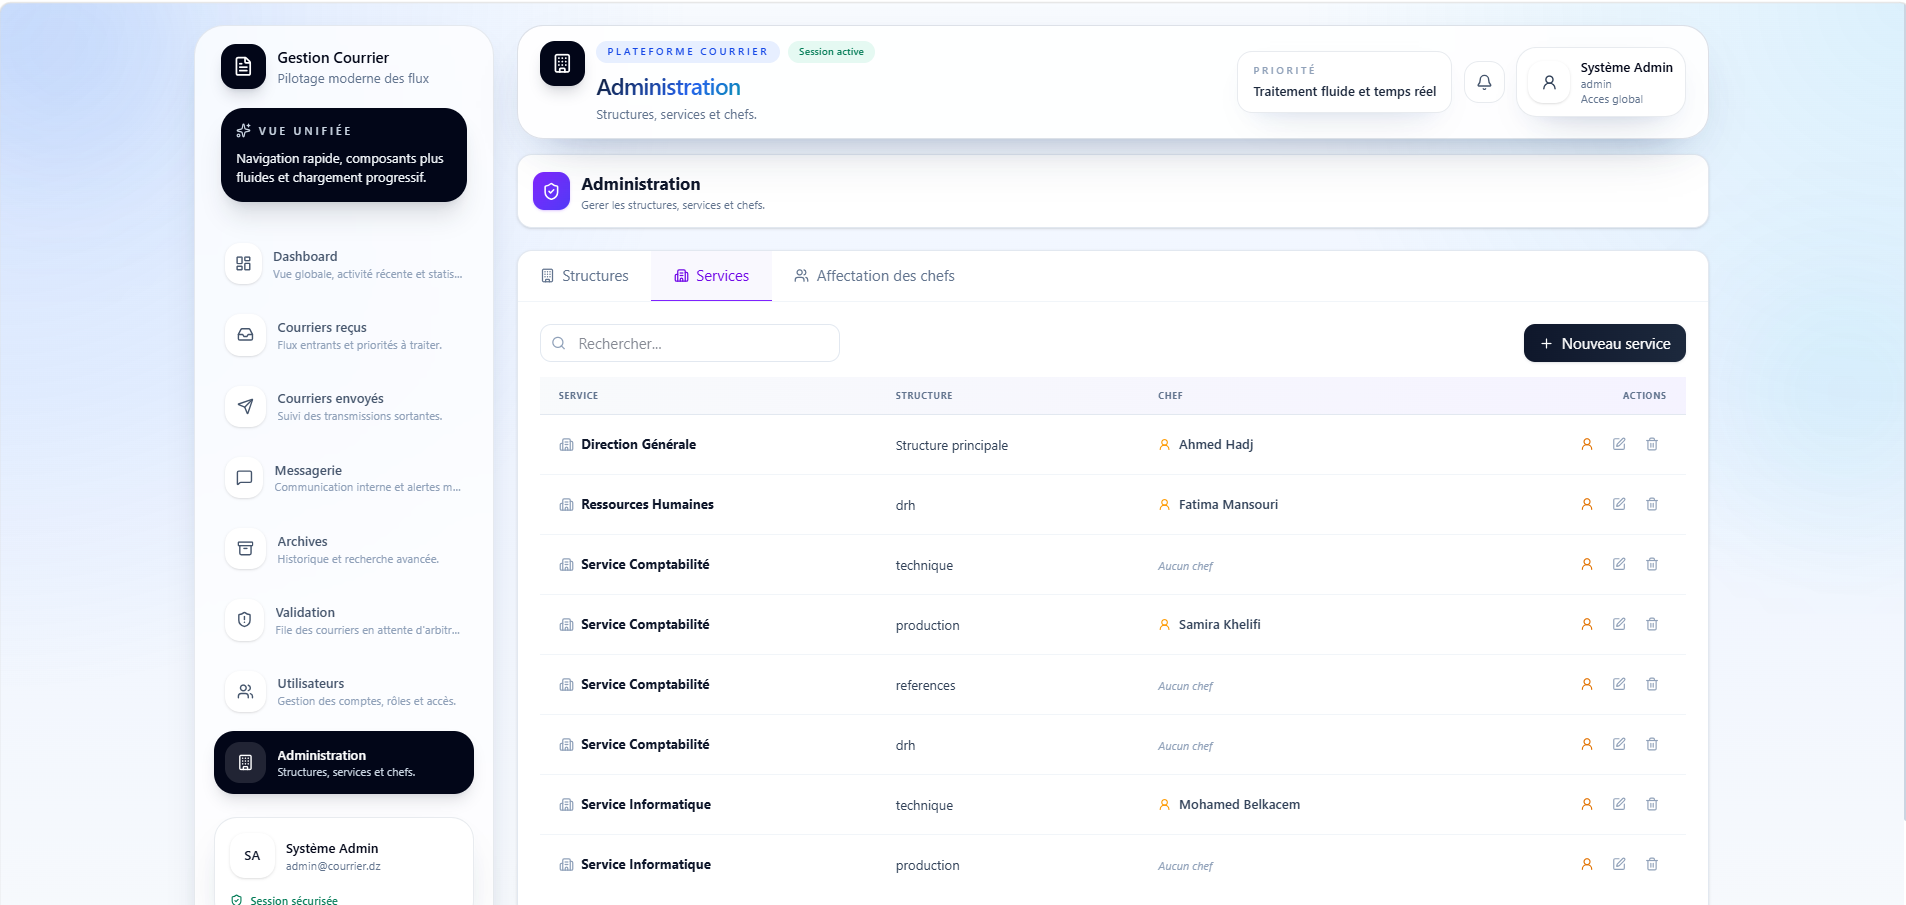
\includegraphics[width=0.92\textwidth,height=0.46\textheight,keepaspectratio]{images/app/services.png}
    \caption{Affichage des services}
    \label{fig:affichage_services}
\end{figure}

\subsubsection{Création d’un service}
\label{subsubsec:creation_service}

La création d’un service permet de définir les différents départements rattachés à une structure. Chaque service peut ensuite être utilisé dans la gestion des courriers, des utilisateurs et des droits d’accès.

\begin{figure}[H]
    \centering
    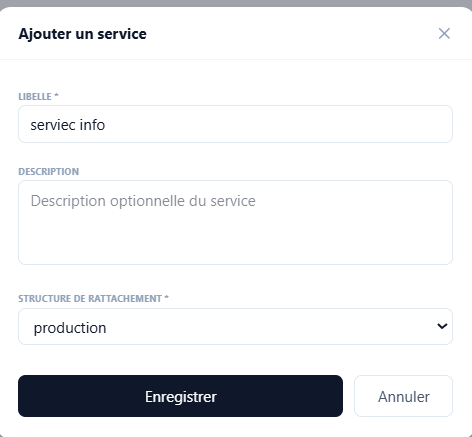
\includegraphics[width=0.88\textwidth,height=0.36\textheight,keepaspectratio]{images/app/services1.png}
    \caption{Création d’un service}
    \label{fig:creation_service}
\end{figure}

\subsubsection{Affectation des responsables}
\label{subsubsec:affectation_responsables}

L’affectation permet d’associer un responsable à une structure ou à un service. Cette étape est importante pour appliquer correctement les règles de validation, de transmission et de consultation des courriers selon le rôle de chaque utilisateur.

\begin{figure}[H]
    \centering
    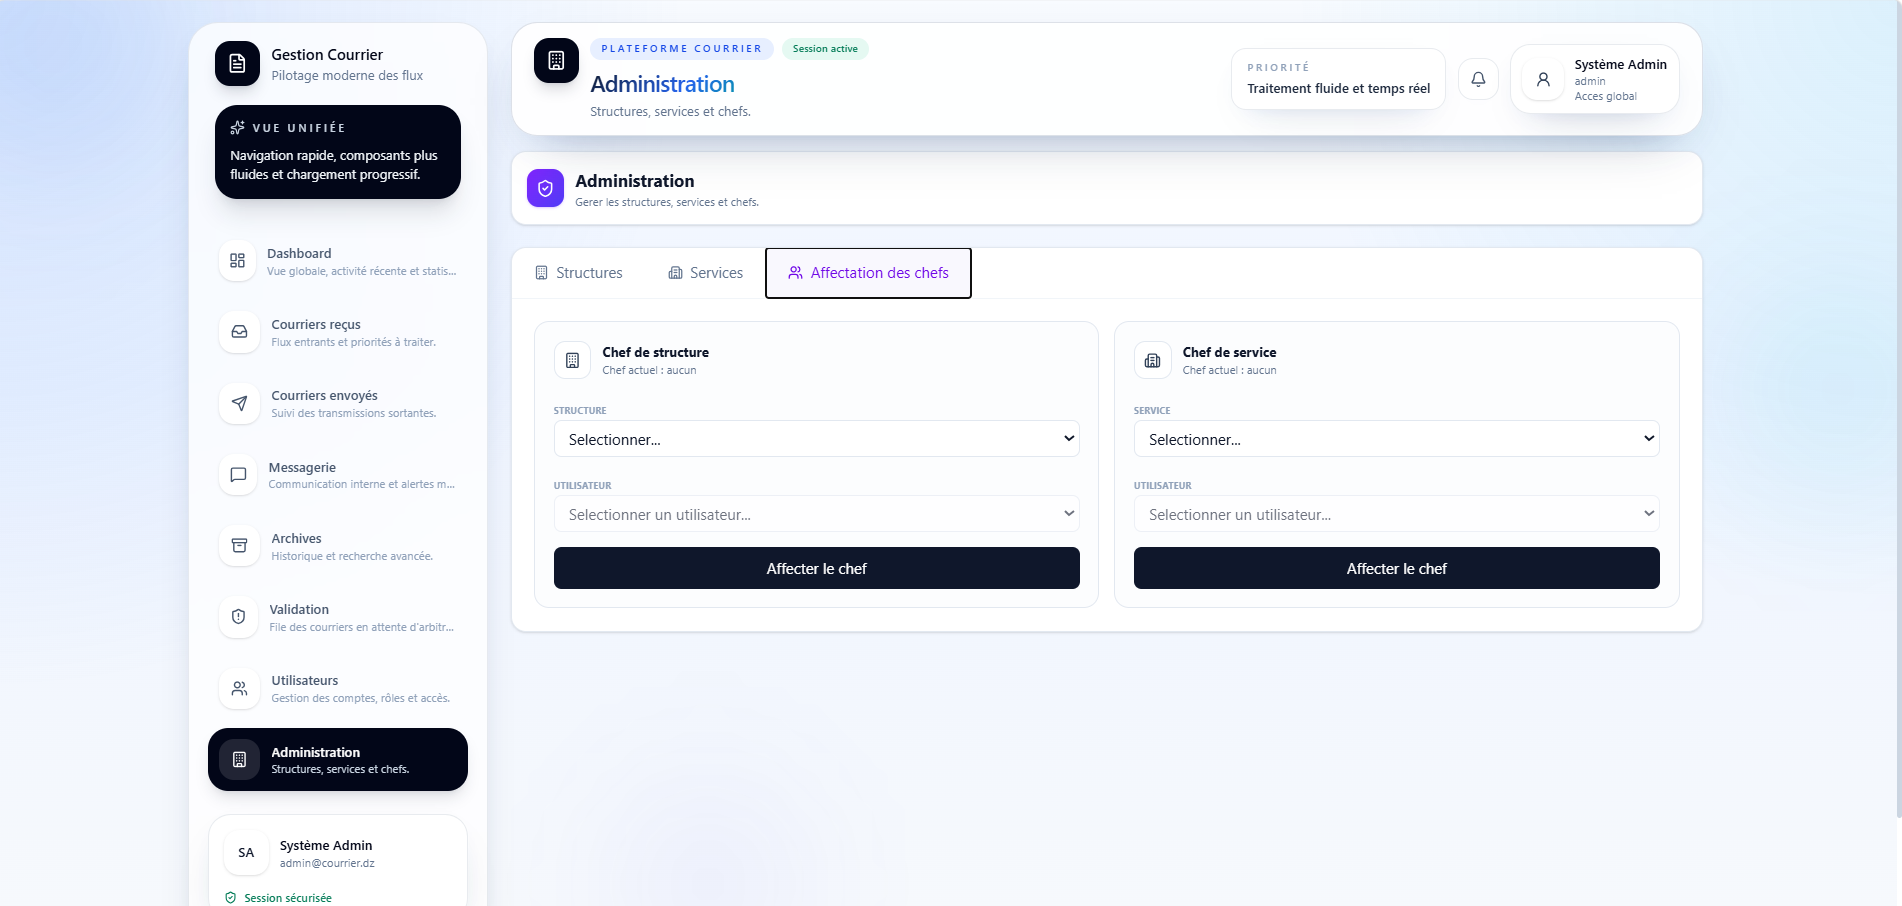
\includegraphics[width=0.88\textwidth,height=0.42\textheight,keepaspectratio]{images/app/affect.png}
    \caption{Affectation des responsables}
    \label{fig:affectation_responsables}
\end{figure}
\section{Conclusion}
\label{sec:conclusion_implementation}

Ce chapitre a présenté les principaux éléments liés à la réalisation de notre application web de gestion de courrier. Nous avons décrit les outils utilisés, l’architecture générale du système, le fonctionnement des échanges entre Laravel et React, ainsi que les principales interfaces développées. Cette étape permet de montrer comment les choix techniques ont été utilisés pour transformer la conception réalisée précédemment en une application fonctionnelle.

% ============================================================================
% Chapitre de sécurité prêt à inclure dans le rapport principal.
%
% Packages nécessaires dans le préambule du rapport principal :
% \usepackage[french]{babel}
% \usepackage{graphicx}
% \usepackage{xcolor}
% \usepackage{booktabs}
% \usepackage{tabularx}
% \usepackage{array}
% \usepackage{float}
% \usepackage{enumitem}
% \usepackage[most]{tcolorbox}
% \usepackage{tikz}
% \usetikzlibrary{arrows.meta,positioning,shapes.geometric,fit,calc}
% ============================================================================

\providecommand{\SecurityAppName}{Gestion Courrier}
\providecommand{\SecurityStack}{Laravel 12, Sanctum, React, API REST}
\providecommand{\SecurityChapterTitle}{Sécurité globale de l'application}

\makeatletter
\@ifundefined{chapter}
  {\section{\SecurityChapterTitle}}
  {\chapter{\SecurityChapterTitle}}
\makeatother
\label{chap:securite-globale}

\section{Introduction}
\label{sec:securite-introduction}

Une application de gestion de courrier administratif manipule des données sensibles : utilisateurs, courriers entrants et sortants, pièces jointes, archives, messages internes, notifications et textes extraits par OCR. La sécurité doit donc être intégrée dès la conception, au niveau de l'architecture, de l'API, des règles d'accès, de la validation des données et de la configuration de production.

Dans ce projet, la sécurité repose sur trois objectifs principaux : confidentialité, intégrité et disponibilité, souvent regroupés sous le sigle CIA dans la terminologie du NIST \cite{nist-cia}. La confidentialité signifie qu'un utilisateur ne consulte que les courriers et fichiers autorisés. L'intégrité garantit qu'un courrier ne peut pas être modifié, validé, transmis ou supprimé hors des règles prévues. La disponibilité vise à maintenir l'application utilisable malgré les erreurs, les traitements lourds ou les tentatives d'abus.

Ces objectifs rejoignent aussi plusieurs risques de l'OWASP Top 10, notamment le contrôle d'accès insuffisant, les injections, les erreurs de configuration et l'utilisation de composants vulnérables \cite{owasp-top10}.

Selon les documents techniques du projet, l'architecture de \SecurityAppName{} repose sur un frontend React de type SPA, une API REST Laravel et une base de données relationnelle \cite{rapport-technique}. Les échanges passent par HTTP/JSON et sont authentifiés avec Laravel Sanctum. Le frontend améliore l'expérience utilisateur, mais la sécurité réelle doit toujours être appliquée côté backend.

\begin{figure}[H]
\centering
\resizebox{0.98\textwidth}{!}{%
\begin{tikzpicture}[
  >=Latex,
  node distance=1.75cm,
  every node/.style={font=\scriptsize},
  box/.style={draw, rounded corners=2pt, align=center, text width=3.15cm, minimum height=1.0cm, fill=gray!5, inner sep=4pt},
  guard/.style={draw, rounded corners=2pt, align=center, text width=3.65cm, minimum height=1.0cm, fill=blue!7, inner sep=4pt},
  edgeLabel/.style={font=\tiny, fill=white, inner sep=1pt}
]
\node[box] (react) {Frontend React\\SPA};
\node[guard, right=of react] (api) {API REST\\Laravel};
\node[guard, right=of api] (policy) {Policies + modèles\\RBAC + confidentialité};
\node[box, right=of policy] (db) {Base de données\\courriers, utilisateurs};
\node[box, below=1.2cm of policy] (storage) {Stockage privé\\pièces jointes + OCR};

\draw[->] (react) -- node[edgeLabel, above=3pt]{HTTPS/JSON} (api);
\draw[->] (api) -- node[edgeLabel, above=3pt]{Sanctum} (policy);
\draw[->] (policy) -- node[edgeLabel, above=3pt]{requêtes contrôlées} (db);
\draw[->] (policy) -- node[edgeLabel, right=3pt]{accès contrôlé} (storage);
\draw[->, dashed] (storage.west) -| node[edgeLabel, near start, below=3pt]{fichiers privés} (api.south);
\end{tikzpicture}%
}
\caption{Principe de défense en profondeur appliqué à l'architecture web}
\label{fig:defense-profondeur}
\end{figure}

\section{Authentification et gestion des utilisateurs}
\label{sec:authentification-gestion-utilisateurs}

L'authentification vérifie l'identité de l'utilisateur avant l'accès aux ressources protégées. Le NIST la définit comme la vérification de l'identité d'un utilisateur, d'un processus ou d'un équipement avant l'autorisation d'accès à un système \cite{nist-auth}. Dans \SecurityAppName{}, cette fonction est assurée par Laravel Sanctum et les sessions Laravel.

Sanctum est adapté aux applications SPA, car il permet d'utiliser des cookies de session avec protection CSRF, sans imposer le stockage d'un jeton sensible dans le navigateur \cite{laravel-sanctum}. Après une connexion réussie, la session doit être régénérée afin de réduire le risque de fixation de session. À la déconnexion, elle est invalidée et le jeton CSRF est renouvelé.

Les mots de passe ne sont jamais stockés en clair. Ils sont hachés avec les mécanismes standards de Laravel, et le champ \texttt{password} doit être masqué dans les réponses JSON. Le modèle utilisateur contient aussi un attribut \texttt{actif}, ce qui permet de désactiver un compte sans le supprimer.

La protection contre la force brute repose sur deux niveaux : la limitation des tentatives, par exemple avec \texttt{throttle:5,1}, et un verrouillage progressif par adresse électronique et adresse IP. Cette combinaison limite les essais automatisés sans bloquer définitivement les utilisateurs légitimes.

Dans un contexte administratif, l'inscription publique représente un risque. Il est donc préférable de désactiver les routes \texttt{/register} en production, ou de créer les comptes avec \texttt{actif=false} jusqu'à validation par un administrateur.

\section{Sécurité native offerte par Laravel}
\label{sec:securite-native-laravel}

Laravel fournit plusieurs protections utiles, mais elles doivent être accompagnées d'une bonne conception applicative. La validation des entrées est assurée par les \texttt{FormRequest}, qui regroupent les règles de format, de présence, de type, de taille, d'existence en base et d'autorisation. Laravel permet aussi de valider les fichiers selon leur extension, leur taille et leur type MIME \cite{laravel-validation}.

L'autorisation côté backend repose sur les \textit{gates} et les \textit{policies}, qui déterminent si un utilisateur peut consulter, modifier ou supprimer une ressource \cite{laravel-authorization}. Dans le projet, ces policies sont complétées par des méthodes métier dans les modèles \texttt{User}, \texttt{Courrier}, \texttt{Message} et \texttt{Archive}. Cela évite qu'un simple identifiant transmis dans une URL donne automatiquement accès au contenu.

Laravel réduit également les risques d'injection SQL grâce à Eloquent ORM et au Query Builder, qui utilisent des requêtes paramétrées. Côté interface, React échappe par défaut le contenu affiché dans le JSX. Ces protections ne dispensent pas de nettoyer les noms de fichiers, d'éviter le HTML brut et de limiter strictement les champs acceptés par l'API.

Enfin, Laravel propose des mécanismes importants comme la protection CSRF, les sessions, le rate limiting, la journalisation et les queues. Ces éléments sont essentiels pour une application web, en particulier lorsqu'elle traite des opérations lourdes comme l'OCR.

\section{Rôles, autorisations et confidentialité des courriers}
\label{sec:roles-autorisations-confidentialite}

Le contrôle d'accès consiste à autoriser ou refuser une demande selon des règles définies. Le NIST le décrit comme un processus permettant de restreindre l'accès aux ressources selon des politiques établies \cite{nist-access}. Dans \SecurityAppName{}, ce contrôle repose sur une logique RBAC enrichie par le périmètre et le niveau de confidentialité.

Les rôles principaux sont \texttt{admin}, \texttt{chef} et \texttt{secretaire}. Les périmètres sont \texttt{general}, \texttt{structure} et \texttt{service}. Ainsi, un chef de service peut exercer ses responsabilités sans obtenir automatiquement les droits d'un chef général.

\begin{table}[H]
\centering
\small
\begin{tabularx}{\textwidth}{lXXXX}
\toprule
\textbf{Profil} & \textbf{Portée} & \textbf{Actions typiques} & \textbf{Limite de sécurité} & \textbf{Contrôle technique} \\
\midrule
Admin & Globale & Administration, suppression, correction & Risque élevé si compte compromis & Middleware admin + policies \\
Chef général & Organisation & Validation et supervision globale & Ne doit pas remplacer l'admin système & Policies + méthodes modèle \\
Chef structure/service & Structure ou service & Validation dans son périmètre & Pas d'accès aux autres structures/services & Filtrage par structure/service \\
Secrétaire & Service ou structure & Création et suivi & Pas de validation finale sensible & Soumission sous contrôle chef \\
\bottomrule
\end{tabularx}
\caption{Synthèse des profils de sécurité et des limites associées}
\label{tab:profils-securite}
\end{table}

La confidentialité ajoute une couche supplémentaire. Même si un utilisateur appartient au bon service ou à la bonne structure, il ne doit pas consulter un courrier dont le niveau de confidentialité dépasse son rang. Le modèle \texttt{Courrier} doit donc comparer le rang de confidentialité du courrier avec celui de l'utilisateur avant d'autoriser l'accès.

\begin{figure}[H]
\centering
\resizebox{0.98\textwidth}{!}{%
\begin{tikzpicture}[
  >=Latex,
  node distance=.75cm,
  every node/.style={font=\small},
  stage/.style={draw, rounded corners, fill=green!6, align=center, minimum width=5.3cm, minimum height=.7cm},
  stop/.style={draw, rounded corners, fill=red!8, align=center, minimum width=4.6cm, minimum height=.75cm}
]
\node[stage] (a) {1. Utilisateur authentifié ?};
\node[stage, below=of a] (b) {2. Ressource dans son périmètre ?};
\node[stage, below=of b] (c) {3. Rôle autorisé pour l'action ?};
\node[stage, below=of c] (d) {4. Rang de confidentialité suffisant ?};
\node[stage, below=of d] (e) {Accès accordé};
\node[stop, right=1.5cm of c] (x) {Refus 403 ou 404};

\draw[->] (a) -- (b);
\draw[->] (b) -- (c);
\draw[->] (c) -- (d);
\draw[->] (d) -- (e);

\draw[->, dashed] (a.east) -- node[above, font=\scriptsize]{non} (x.north west);
\draw[->, dashed] (b.east) -- node[above, font=\scriptsize]{hors périmètre} (x.west);
\draw[->, dashed] (c.east) -- node[below, font=\scriptsize]{rôle refusé} (x.west);
\draw[->, dashed] (d.east) -- node[below, font=\scriptsize]{rang insuffisant} (x.south west);
\end{tikzpicture}%
}
\caption{Chaîne de décision pour la consultation d'un courrier}
\label{fig:decision-acces}
\end{figure}

La figure~\ref{fig:decision-acces} illustre les contrôles appliqués avant la consultation d'un courrier. Lorsqu'une condition échoue, la demande est refusée avec une réponse adaptée : \texttt{403} si l'accès est interdit, ou \texttt{404} si la ressource ne doit pas être révélée.

Cette approche répond à deux risques importants : le contrôle d'accès cassé dans les applications web et le \textit{Broken Object Level Authorization} dans les API \cite{owasp-api}. Pour éviter l'IDOR, chaque route qui reçoit un identifiant de courrier, message, archive ou pièce jointe doit vérifier les droits sur l'objet avant de retourner les données.

\section{Sécurité côté web, API et fichiers}
\label{sec:securite-web-api-fichiers}

Les routes API sensibles doivent rester protégées par \texttt{auth:sanctum}. Cela concerne la consultation des courriers, les détails, la validation, la transmission, l'archivage, la messagerie, les utilisateurs, les notifications et l'OCR. Masquer un bouton côté React ne suffit pas : chaque action doit être contrôlée côté Laravel, car un utilisateur peut appeler directement un endpoint.

Côté web, trois points sont prioritaires. La configuration CORS doit être stricte en production, avec uniquement les origines officielles de l'application. L'application doit être servie en HTTPS, avec des cookies \texttt{Secure}, \texttt{HttpOnly} et \texttt{SameSite}. Les en-têtes de sécurité doivent aussi être activés, notamment \texttt{Content-Security-Policy}, \texttt{Strict-Transport-Security}, \texttt{X-Frame-Options}, \texttt{X-Content-Type-Options}, \texttt{Referrer-Policy} et \texttt{Permissions-Policy}.

Les fichiers représentent une zone sensible, car les pièces jointes peuvent contenir des informations confidentielles ou des contenus malveillants. Les formats acceptés doivent être limités, avec contrôle du type MIME, de la taille et du nombre maximal de fichiers. Le stockage doit rester privé, par exemple dans \texttt{storage/app/private}, et le téléchargement doit passer par une route Laravel qui vérifie les droits de consultation.

Il faut éviter les liens directs vers \texttt{/storage/...} pour les documents sensibles. Ces liens peuvent contourner la logique d'autorisation de l'application si le dossier est exposé publiquement.

Le module OCR augmente aussi la surface d'attaque, car il traite des PDF, images et documents Word avec des outils externes. Il doit fonctionner avec des limites de mémoire, de temps et de taille de fichier. Les erreurs techniques doivent être journalisées sans être affichées directement à l'utilisateur. Le texte extrait par OCR doit hériter des mêmes règles d'accès que le courrier et ses pièces jointes \cite{documentation-ocr}.

\begin{table}[H]
\centering
\small
\begin{tabularx}{\textwidth}{lXl}
\toprule
\textbf{Zone technique} & \textbf{Protection recommandée} & \textbf{Risque réduit} \\
\midrule
API REST & \texttt{auth:sanctum}, policies, validation objet par objet & IDOR, actions non autorisées \\
Sessions & Régénération, cookies \texttt{HttpOnly}, \texttt{Secure}, \texttt{SameSite} & Vol ou fixation de session \\
CORS & Origines officielles uniquement en production & Appels cross-origin abusifs \\
Fichiers & MIME, taille, stockage privé, téléchargement contrôlé & Fuite ou dépôt malveillant \\
OCR & Queue, limites ressources, outils à jour, erreurs filtrées & Déni de service ou exposition interne \\
Headers & CSP, HSTS, X-Frame-Options, X-Content-Type-Options & XSS, clickjacking, sniffing \\
\bottomrule
\end{tabularx}
\caption{Synthèse des protections web, API et fichiers}
\label{tab:protections-web}
\end{table}

Le tableau~\ref{tab:protections-web} résume les protections principales à appliquer pour réduire les risques liés à l'API, aux sessions, aux fichiers, à l'OCR et à la configuration web.

\section{Conclusion}
\label{sec:securite-conclusion}

La sécurité de \SecurityAppName{} repose sur une défense en profondeur. Elle combine l'authentification par session protégée, l'autorisation par rôles et périmètres, la confidentialité par rang, la validation des entrées, le stockage privé des fichiers, le rate limiting, le contrôle des notifications temps réel et les tests automatisés.

Cette stratégie correspond aux besoins d'une application administrative, car elle prend en compte la hiérarchie de l'organisation, la sensibilité des documents et les risques propres aux applications web modernes.

La sécurité ne se limite donc pas à la page de connexion. Elle doit être présente dans les routes API, les policies, les modèles, les requêtes de validation, le stockage des fichiers et la configuration serveur. Les derniers points à renforcer concernent surtout la mise en production : gestion des secrets, configuration CORS, en-têtes HTTP, suppression des routes de test, durée des tokens, logs et durcissement du module OCR.

\bibliographystyle{plain}

\begin{thebibliography}{99}

\bibitem{bissonnette2012}
Natalie Bissonnette,
\textit{Gestion des courriels : stratégies, technologies et bonnes pratiques},
Archives, vol. 44, no. 1, pp. 77--113, 2012--2013.
Disponible sur :
\url{https://bibliopiaf.ebsi.umontreal.ca/bibliographie/HSIFPFA9/download/5TI3E5XK/Bissonnette%20-%202012%20-%20Gestion%20des%20courriels%20%20strat%C3%A9gies%2C%20technologies%20e.pdf}

\bibitem{piaf}
PIAF Archives,
\textit{Définition du courrier électronique},
Disponible sur :
\url{https://www.piaf-archives.org/sites/default/files/bulk_media/m07bs7/co/07B_section7_7.html}

\bibitem{piafgestion}
PIAF Archives,
\textit{La gestion des courriels et des documents interactifs},
Disponible sur :
\url{https://www.piaf-archives.org/sites/default/files/bulk_media/m07bs7/co/07B_section7_11.html}

\bibitem{technoscience}
Techno-Science,
\textit{Courrier électronique},
Disponible sur :
\url{https://www.techno-science.net/glossaire-definition/Courrier-electronique.html}

\bibitem{maarch}
Maarch,
\textit{Livre blanc GEC 2025},
Disponible sur :
\url{https://maarch.com/wp-content/uploads/livre_blanc_GEC_2025.pdf}

\bibitem{scribd}
Scribd,
\textit{Exposé sur le courrier électronique},
Disponible sur :
\url{https://fr.scribd.com/document/710843534/Expose-Sur-Le-Courrier-Electronique}
\bibitem{laravel}
Laravel,
\textit{Laravel -- The PHP Framework for Web Artisans},
Disponible sur :
\url{https://laravel.com/}

\bibitem{laraveldocs}
Laravel,
\textit{Laravel Documentation},
Disponible sur :
\url{https://laravel.com/docs/12.x/documentation}
\bibitem{laravel_eloquent}
Laravel,
\textit{Eloquent: Getting Started -- Laravel Documentation},
Disponible sur :
\url{https://laravel.com/docs/12.x/eloquent}

\bibitem{laravel_relationships}
Laravel,
\textit{Eloquent: Relationships -- Laravel Documentation},
Disponible sur :
\url{https://laravel.com/docs/12.x/eloquent-relationships}

\bibitem{laravel_mutators}
Laravel,
\textit{Eloquent: Mutators and Casting -- Laravel Documentation},
Disponible sur :
\url{https://laravel.com/docs/12.x/eloquent-mutators}
\bibitem{laravel_sanctum}
Laravel,
\textit{Laravel Sanctum -- Laravel Documentation},
Disponible sur :
\url{https://laravel.com/docs/12.x/sanctum}

\bibitem{laravel_reverb}
Laravel,
\textit{Laravel Reverb -- Real-time WebSocket Server},
Disponible sur :
\url{https://reverb.laravel.com/}


\bibitem{react}
React,
\textit{React -- The library for web and native user interfaces},
Disponible sur :
\url{https://react.dev/}

\bibitem{react_router}
React Router,
\textit{Routing -- React Router Documentation},
Disponible sur :
\url{https://reactrouter.com/start/library/routing}

\bibitem{axios}
Axios,
\textit{Axios -- Promise based HTTP client},
Disponible sur :
\url{https://axios.rest/}
\bibitem{tailwind}
Tailwind CSS,
\textit{Tailwind CSS -- Utility-first CSS framework},
Disponible sur :
\url{https://tailwindcss.com/docs/utility-first}
\bibitem{plantuml}
PlantUML,
\textit{Guide de référence du langage PlantUML},
Disponible sur :
\url{https://pdf.plantuml.net/1.2020.22/PlantUML_Language_Reference_Guide_fr.pdf}

\bibitem{xampp}
Apache Friends,
\textit{XAMPP Installers and Downloads for Apache Friends},
Disponible sur :
\url{https://www.apachefriends.org/fr/index.html}

\bibitem{mariadb}
MariaDB Foundation,
\textit{MariaDB en bref},
Disponible sur :
\url{https://mariadb.org/fr/}

\bibitem{apache}
The Apache Software Foundation,
\textit{The Apache HTTP Server Project},
Disponible sur :
\url{https://httpd.apache.org/}

\bibitem{tesseract}
Tesseract OCR,
\textit{Tesseract User Manual},
Disponible sur :
\url{https://tesseract-ocr.github.io/tessdoc/}

\bibitem{rest_api}
Red Hat,
\textit{Une API REST, qu'est-ce que c'est ?},
Disponible sur :
\url{https://www.redhat.com/fr/topics/api/what-is-a-rest-api}
\bibitem{laravel_lifecycle}
Laravel,
\textit{Request Lifecycle -- Laravel Documentation},
Disponible sur :
\url{https://laravel.com/docs/12.x/lifecycle}

\bibitem{laravel_responses}
Laravel,
\textit{HTTP Responses -- Laravel Documentation},
Disponible sur :
\url{https://laravel.com/docs/12.x/responses}

\bibitem{axios}
Axios,
\textit{Axios -- Promise based HTTP client},
Disponible sur :
\url{https://github.com/axios/axios}

\bibitem{mdn_json}
MDN Web Docs,
\textit{Working with JSON},
Disponible sur :
\url{https://developer.mozilla.org/en-US/docs/Learn_web_development/Core/Scripting/JSON}

\bibitem{bitnami_redmine}
Bitnami,
\textit{Run Redmine in the Cloud},
Disponible sur :
\url{https://docs.bitnami.com/general/how-to/use-redmine/}

\bibitem{redmine_overview}
Redmine,
\textit{Overview},
Disponible sur :
\url{https://www.redmine.org/}

\bibitem{redmine_workflow}
Redmine,
\textit{Redmine Issue Tracking Setup},
Disponible sur :
\url{https://www.redmine.org/projects/redmine/wiki/RedmineIssueTrackingSetup}

\bibitem{redmine_rest_api}
Redmine,
\textit{REST API},
Disponible sur :
\url{https://www.redmine.org/projects/redmine/wiki/Rest_api}
\bibitem{omg_uml}
Object Management Group,
\textit{Unified Modeling Language},
Disponible sur :
\url{https://www.omg.org/UML/}

\bibitem{omg_uml_spec}
Object Management Group,
\textit{About the Unified Modeling Language Specification Version 2.5.1},
Disponible sur :
\url{https://www.omg.org/spec/UML/2.5.1/About-UML/}

\bibitem{ibm_uml_diagrams}
IBM,
\textit{UML diagrams},
Disponible sur :
\url{https://www.ibm.com/docs/en/dma?topic=diagrams-uml}

\bibitem{ibm_use_case}
IBM,
\textit{Use-case diagrams in UML modeling},
Disponible sur :
\url{https://www.ibm.com/docs/en/dma?topic=diagrams-use-case}

\bibitem{redmineup_themes_2025}
RedmineUP, \textit{5 Best Themes for Redmine in 2025}, publié le 17 février 2025. Disponible sur : 
\url{https://www.redmineup.com/pages/blog/best-redmine-theme-2025}. Consulté le 13 mai 2026.

\bibitem{patel_laravel_lifecycle}
Parixit Patel, \textit{Laravel Request Lifecycle}, DEV Community, publié le 15 juillet 2020. Disponible sur :
\url{https://dev.to/patelparixit07/laravel-request-lifecycle-195e}. Consulté le 13 mai 2026.
\bibitem{nist-cia}
NIST CSRC, \textit{Confidentiality, Integrity, Availability}, Glossary,
\url{https://csrc.nist.gov/glossary/term/confidentiality_integrity_availability}.

\bibitem{nist-auth}
NIST CSRC, \textit{Authentication}, Glossary,
\url{https://csrc.nist.gov/glossary/term/authentication}.

\bibitem{nist-access}
NIST CSRC, \textit{Access Control}, Glossary,
\url{https://csrc.nist.gov/glossary/term/access_control}.

\bibitem{laravel-sanctum}
Laravel Documentation, \textit{Laravel Sanctum - SPA Authentication},
\url{https://laravel.com/docs/12.x/sanctum}.

\bibitem{laravel-validation}
Laravel Documentation, \textit{Validation and Form Requests},
\url{https://laravel.com/docs/12.x/validation}.

\bibitem{laravel-authorization}
Laravel Documentation, \textit{Authorization - Gates and Policies},
\url{https://laravel.com/docs/12.x/authorization}.

\bibitem{owasp-top10}
OWASP, \textit{OWASP Top 10:2021},
\url{https://owasp.org/Top10/2021/}.

\bibitem{owasp-api}
OWASP, \textit{OWASP API Security Top 10 - 2023},
\url{https://owasp.org/API-Security/editions/2023/en/0x11-t10/}.

\bibitem{rapport-technique}
Documents internes du projet, \textit{Rapport technique et sécurité - application Gestion Courrier}, 2026.

\bibitem{rapport-securite}
Documents internes du projet, \textit{Rapport de sécurité globale de l'application de gestion de courrier}, 2026.

\bibitem{documentation-ocr}
Documents internes du projet, \textit{Module OCR et traitement automatique des documents}, 2026.

\end{thebibliography}



\end{document}
